\documentclass[a4paper]{article}
\usepackage[utf8]{inputenc}
\usepackage[spanish]{babel}
% \usepackage{hyperref}
\usepackage{graphicx}
\usepackage{float}


\title{
\textsc{\normalsize Interacción Persona-Computadora} \\
\vspace{1cm}
\hrule
\vspace{0.4cm}
Sintonízame Informe % poner aquí el título del documento
\vspace{0.5cm}
\hrule
} 
\author{Sergio Alonso Pascual \\ Adrián Arroyo Calle \\ Irene Caldelas Fernández \\ Cristina de la Torre Cáceres}
\date{Mayo 2018}


\begin{document}

\maketitle

\tableofcontents

\listoffigures

\pagebreak

\section{Introducción}

En el mundo actual, los usuarios quieren poder escuchar sus programas de radio en cualquier momento, previamente grabados. Con este nuevo medio de comunicación conocido como \textit{podcast}, han surgido diferentes aplicaciones que buscan ser amigables con el usuario y que actúen de forma lo más transparente posible, rompiendo la barrera entre creadores de contenido y consumidores. De ahí surge, Sintonízame, una aplicación multidispositivo que permite a los usuarios escuchar sus podcasts preferidos de sus locutores preferidos cuando quieran y donde quieran, con la máxima calidad posible.

\begin{center}
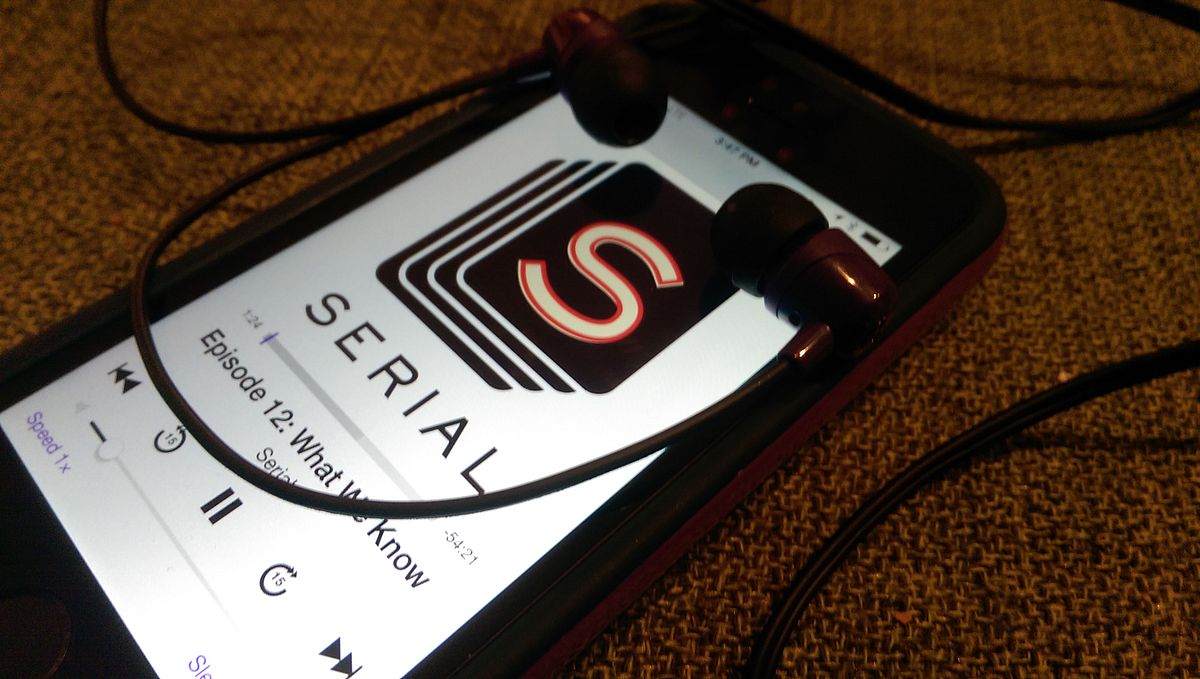
\includegraphics[width=0.7\columnwidth]{Podcast.jpg}
\end{center}

\section{Requisitos funcionales de la aplicación}

La aplicación diseñada, permite escuchar podcasts, suscribirse a canales creadores de podcasts para recibir novedades, crear playlists de podcasts y mostrar sugerencias de nuevos podcasts.

\section{Prototipado de bajo coste}

Para realizar las primeras pruebas de usabilidad, se ha diseñado un prototipo con materiales reciclados y de bajo coste.

Para el prototipo de Sintonízame hemos hecho un teléfono falso, al que le vamos cambiando las pantallas con cartulinas. El teléfono falso está hecho con una caja de cartón (que en tiempos pasados era de chocolate) al que se le ha recortado una ventana de tamaño amplio, para simular las pantallas táctiles de los \textit{smartphones} actuales. Aunque más voluminoso que un teléfono real, la experiencia en la mano es similar y el peso es parecido. Las pantallas, cuyas dimensiones exactas son de 9x16,5 centímetros, se ajustan a la ventana de la maqueta, de 9x15,5. Se deja un centímetro para poder cambiar entre pantallas con mayor facilidad. Las cartulinas aportan consistencia extra ya que no se doblan con tanta facilidad.

Además, la caja dispone de una ranura para introducir los diferentes teclados que la aplicación puede pedir para que el usuario introduzca datos. Estos teclados, solo aparecen al encontrarse un campo de texto, para no malgastar espacio de la pantalla innecesariamente.

Para el prototipo hemos diseñado un logo con lettering, salvo eso, que es por motivos estéticos, el resto de la aplicación usa tipografías claras para que los usuarios no deban esforzarse mucho en leer los botones y opciones.

La interfaz consta de una barra inferior que permite acceder rápidamente a las acciones más comunes, la barra no tiene más de 3 opciones (Mi Perfil, Buscar y Suscripciones) ya que buscamos sencillez. La ley de Fitts además nos indica que el lugar adecuado para un menú de este tipo es justamente en un borde de la pantalla. El resto de la pantalla es la acción principal que se esté realizando: escuchar un podcast, revisar las sugerencias, encontrar las novedades,...

En estas pantallas se prima el contenido visual y unos pocos botones de acción, grandes, muy en línea con otras aplicaciones similares de reproducción de contenido multimedia: reproducir/pausa, ajustes de sonido (volumen, calidad, etc). En la pantalla de novedades existe una barra superior de búsqueda, esta incluye a su vez un botón para activar filtros de búsqueda, referentes a género, idioma, fecha, ...

Inicialmente diseñamos los bocetos pensando en una interfaz en horizontal, acorde al resto de dispositivos con los que es compatible la aplicación, posteriormente decidimos que en un teléfono era mucho más conveniente soportar el modo vertical en primer (y de momento único) lugar. Esto es debido a que la mayoría de aplicaciones trabajan en ese modo y el launcher desde el que se lanza la aplicación también suele ser vertical. Bocetos en \ref{bocetos}

\section{Test}

El día 18 de mayo procedemos al test con usuarios ajenos al proyecto. Durante las 8 rondas, vamos analizando aspectos de la usabilidad de la aplicación, con algunas sorpresas en los resultados. 

El puesto de facilitador iba rotando entre todos los miembros del equipo y era el único que podía hablar con el usuario, proponiéndole tareas a realizar y sugiriendo, pero nunca dando la solución a la tarea.

El facilitador seguía el guion expuesto en la sección 4.1

\subsection{Guion del facilitador}

Se pretende observar la usabilidad del prototipo de la aplicación Sintonízame, una aplicación novedosa para escuchar podcasts. En este test se probará la versión diseñada para teléfonos móviles, a través de una maqueta que refleja los menús y pantallas que se han definido inicialmente.

El \textbf{facilitador} muestra la maqueta por primera vez al usuario que va a realizar el test. Se le recuerda al usuario que no está siendo examinado, que todo lo que diga va a estar bien, si algo no es evidente, es nuestro fallo. También se le anima a expresar cualquier pensamiento que tenga en cualquier momento. 

La prueba comienza con el facilitador diciendo el nombre de la aplicación, mostrando una pantalla principal y preguntando al usuario: ¿De qué crees que va esta aplicación? 

A continuación el facilitador le explicará brevemente la finalidad de la aplicación, de forma rápida, en 10 segundos, a modo de \textit{elevator pitch}. 

La primera tarea que se le pedirá al usuario es que intente \textbf{iniciar sesión en la aplicación}. El facilitador no ayudará al usuario que realiza el test salvo que el usuario se encuentre realmente perdido. La decisión final de ayudar al usuario con pistas será en todo caso del facilitador. Al acabar la tarea con éxito, el facilitador le agradece su colaboración. Durante esta tarea tenemos que observar el tiempo que tarda, si la interfaz le resulta similar a otras conocidas, errores que haya podido cometer, tanto intencionadamente como accidentalmente.

La segunda tarea consistirá en pedir al usuario que \textbf{encuentre novedades en el podcast de ejercicio}. Una vez hecho eso, tendrá que escuchar un podcast y ajustar el audio en modo Estéreo. Se repetirá el mismo procedimiento que en la primera tarea por parte del facilitador.

La tercera tarea consistirá en pedir al usuario que \textbf{busque un podcast que hable sobre teoría del color}. Para ello el facilitador le animará a usar filtros de búsqueda, sabiendo que el podcast durá más de 10 minutos y que es en español.

A continuación, se le harán unas cuantas preguntas rápidas:
\begin{itemize}
\item ¿Sabrías crear una playlist?
\item ¿Sabrías editar tu propio perfil?
\item ¿Podrías suscribirte a un canal recomendado?
\end{itemize}

Finalmente, el facilitador pedirá al usuario una opinión general sobre la aplicación. Es mucho más útil un comentario negativo, que uno positivo.

\section{Resultados}

De las pruebas realizadas pudimos extraer información valiosa.

\subsection{Organización general}

En general no hubo demasiados problemas con la organización de la aplicación propuesta. Las pantallas eran accesibles fácilmente. Sin embargo, al menos uno de los usuarios, en la tarea de buscar, no usó la lupa, sino que decidió explorar manualmente. Este usuario realizó la tarea con éxito, aunque tardó algo más de tiempo.

Otros usuarios criticaron la falta de botón para volver atrás. A pesar de que la movilidad de la aplicación era accesible desde los botones propuestos. Hemos de recalcar que la mayoría de usuarios se lanzaron a la aventura a clickar botones sin detenerme a pensar en que estaban haciendo, se guían por la necesidad de tener el control sobre la aplicación.

\subsection{Login}

La mayoría de los usuarios reconocieron el login como algo estándar, presente en otras aplicaciones de igual forma. No obstante, se criticó que no hubiese botón específico para iniciar sesión. En la evaluación del prototipo con usuarios reales se implementó al pulsar en el teclado el tick de confirmación de que se había acabado de escribir.

Siguiendo las pautas del diseño iterativo recogimos todos estos datos e implementamos un botón de "Aceptar" para acceder a la aplicación una vez introducidos los datos.

\subsection{Perfil}

Se criticó la falta de un botón específico para editar. El hecho de que el perfil sea editable desde el principio no es evidente.

Una de las opciones era que a través de manipulación directa el usuario clickara en los campos de texto que quisiera editar. Pero como comprobamos esto no era demasiado intuitivo. Por esto decidimos implementar un icono basado en un lápiz escribiendo para comenzar a modificar los datos del perfil. 

\subsection{Búsqueda y recomendaciones}

Nadie usó el botón de filtros, ya que realmente la mayoría de la gente simplemente buscaba por el nombre del podcast.

El icono de los podcast influyó mucho en la búsqueda. En concreto, el podcast de decoración tenía un bote de pintura dibujado, sin embargo mucha gente no relacionó ambos conceptos y se quedaron mucho tiempo en la pantalla pensando cuál sería el podcast de decoración o ponían en el buscador "Decoración" como tal. En este caso se podría haber hecho a través de los filtros donde había una opción de tipo.

El canal al que pedíamos que se suscribieran formaba parte de una top de tres canales de los cuales Silvia estaba suscrita a dos de ellos siendo el de decoración el único que mostraba la suscripción.

\subsection{Reproducción}

Aquí una parte importante de los usuarios tuvieron que pensar que botón ajustaría las opciones de sonido, confundiéndolo con el de volumen. Aunque normalmente ellos se daban cuenta de que estaban equivocados al ver el icono verdadero. Ningún usuario cambió el volumen usando los botones físicos del dispositivo. No eran visibles ya que no resaltaban respecto a la estructura de prisma del teléfono.

\subsection{Suscripciones}

En esta pantalla apenas se detectaron problemas.Los usuarios supieron detectar que los canales a los cuales estaban suscritos se encontraba dentro del botón de suscripciones. Dentro de este supieron identificar aquellos canales que tenían notificaciones de podcasts nuevos y acceder a ellos. 

\subsection{Detalles del Podcast}

No todos los usuarios fueron capaces de adivinar que pulsando sobre la descripción de un episodio en concreto se iniciaba su reproducción. Hubo usuarios que pulsaron \textit{Reproducir todo} y fueron pasando con las flechas individualmente entre todos los episodios hasta llegar al correcto. Podemos deducir de esto que en el modelo mental de los usuarios no concebían la aplicación como una app para un smartphone obviando la tactilidad de este.

\section{Propuestas de mejora}

Dados los resultados del test se proponen las siguientes mejoras para mejorar la usabilidad de la aplicación:

\begin{itemize}
\item Añadir botón de Iniciar Sesión en la pantalla de inicio de sesión
\item Marcar de forma clara que los elementos de la pantalla perfil son editables
\item Prestar atención a los iconos de los podcast
\item Aportar información adicional en la pantalla de búsqueda relativa a la temática
\item Juntar los botones de volumen y ajustes de sonido para evitar confusión, podrían incluso unirse
\item Marcar de alguna forma que al pulsar sobre un episodio se puede empezar a reproducir, como un icono de play al lado de ellos.
\end{itemize}

\subsection{Participantes en el test de usabilidad}

A algunos usuarios le surgieron dudas respecto a la utilización de los botones inferiores  dando lugar a confusiones a la hora de moverse por la interfaz. La gente no lo veía como 3 botones independientes si no como un indicador de la vista en la que se encuentran.\\

Reiteramos que muchos usuarios alabaron la intuitividad de la interfaz pero la mayoría de ellos coincidieron en que el bote de pintura no era muy fácil relacionarlo con el canal de decoración así como el nombre que le dimos.\\

Algunos de ellos se sintieron muy confundidos a la hora de utilizar el teclado del móvil para introducir los datos, mucho de ellos tomaron el control de ordenador y lo hicieron por cuenta propia. De nuevo nos encontramos en la tesitura de que no lo veían como una aplicación para un dispositivo táctil.

\section{Conclusiones de los diseñadores}

Tras haber realizado el test de evaluación con usuarios nos dimos cuenta de varias cosas que comentamos en puntos anteriores, pero también  de otras relacionadas con el papel de observador y ordenador.

Intentamos tener todas las posibles decisiones del usuario en cuenta, para ello teníamos una gran cantidad de post-it con las diferentes opciones para cada una de las vistas. Esto acabó ocasionando un lio de qué post-it iba en donde, cuando y por qué haciendo un poco más lento la evaluación del prototipo.

Otra de las cosas de las que nos dimos cuenta y hemos mencionado es el hecho de que algunos usuarios no relacionaban el botón de la lupa con buscar. A la hora de buscar estas metáforas nos guiamos por la mayoría de aplicaciones que usan esto para buscar y creímos que al ser una metáfora tan utilizada los usuarios no tendrían problemas en darse cuenta de ello.

Algo que han coincidido la mayoría de usuarios es que el logotipo no era intuitivo, algunos eran incapaces de leer el nombre de la aplicación y otros no veían la relación del logo (una taza de café/té con un antena de radio) con el tipo de aplicación.

\section{Fases del prototipo con imágenes}
\label{Fases del prototipo}

\subsection{Tarea 1}
\begin{center}
\begin{figure}[H]
\centering
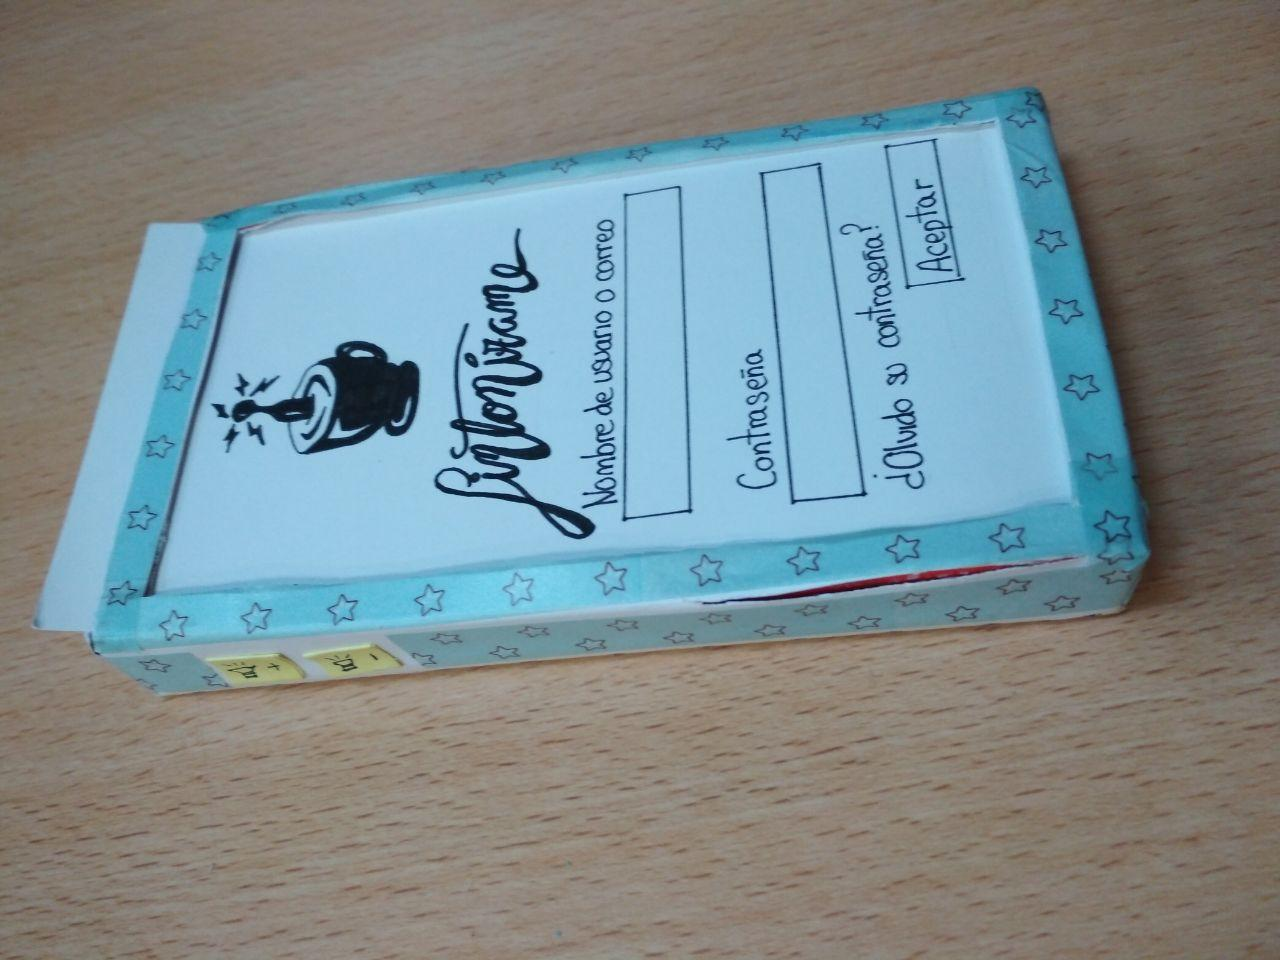
\includegraphics[height=0.4\columnwidth,angle=-90]{T1-1.jpg}
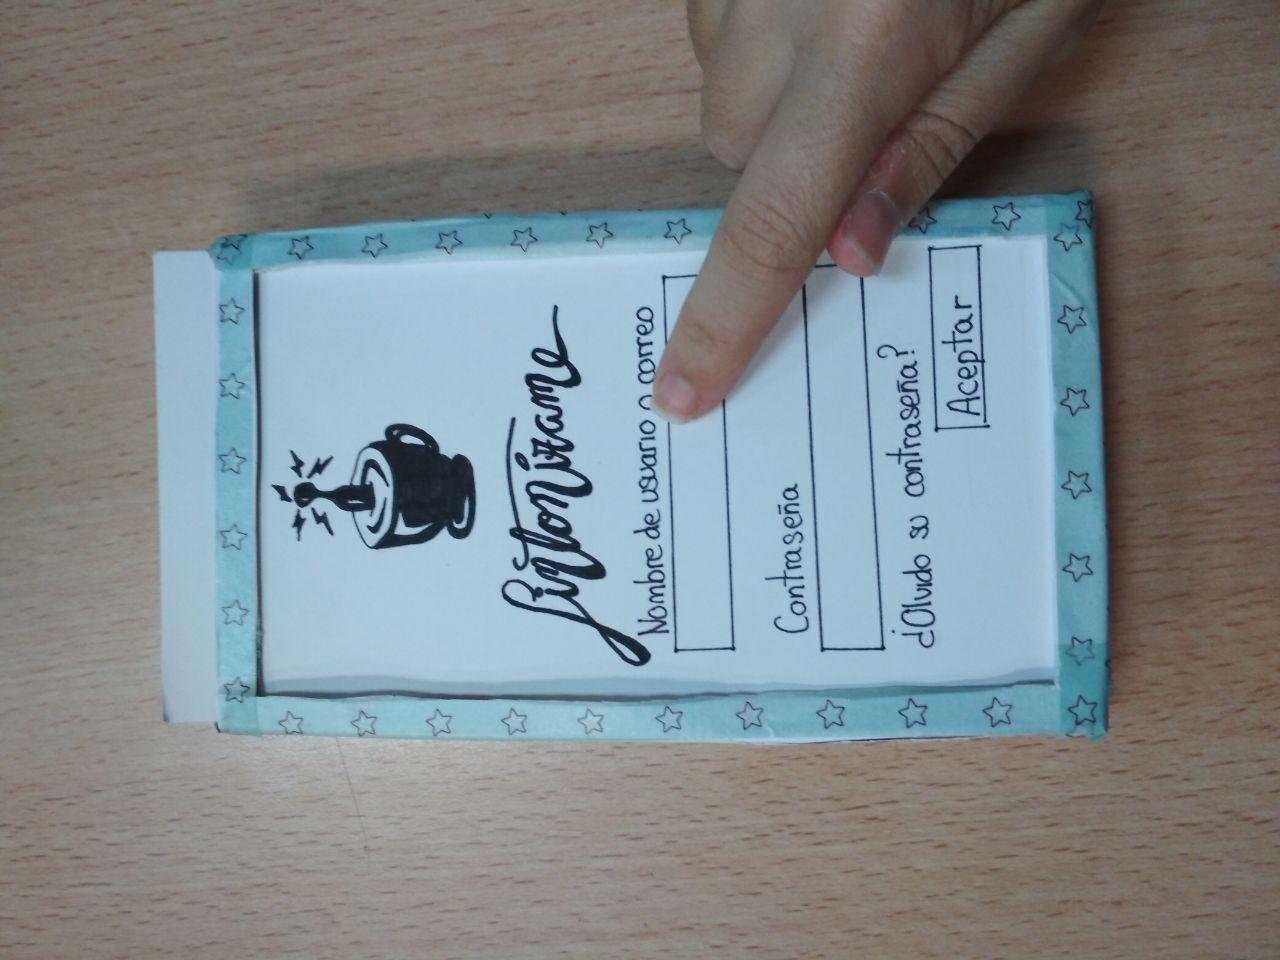
\includegraphics[height=0.4\columnwidth,angle=-90]{T1-2.jpg}
\caption{Pantalla de inicio de sesión}
\label{fig:t1-1}
\end{figure}
Contamos con un dispositivo en cartón que actuará como smartphone y contendrá las distintas vistas. En el lateral de este podremos ver dos botones que harán de ajustes de volumen. Al principio mostramos una vista que permite introducir tus datos para acceder a tu cuenta en la app.
\begin{figure}[H]
\centering
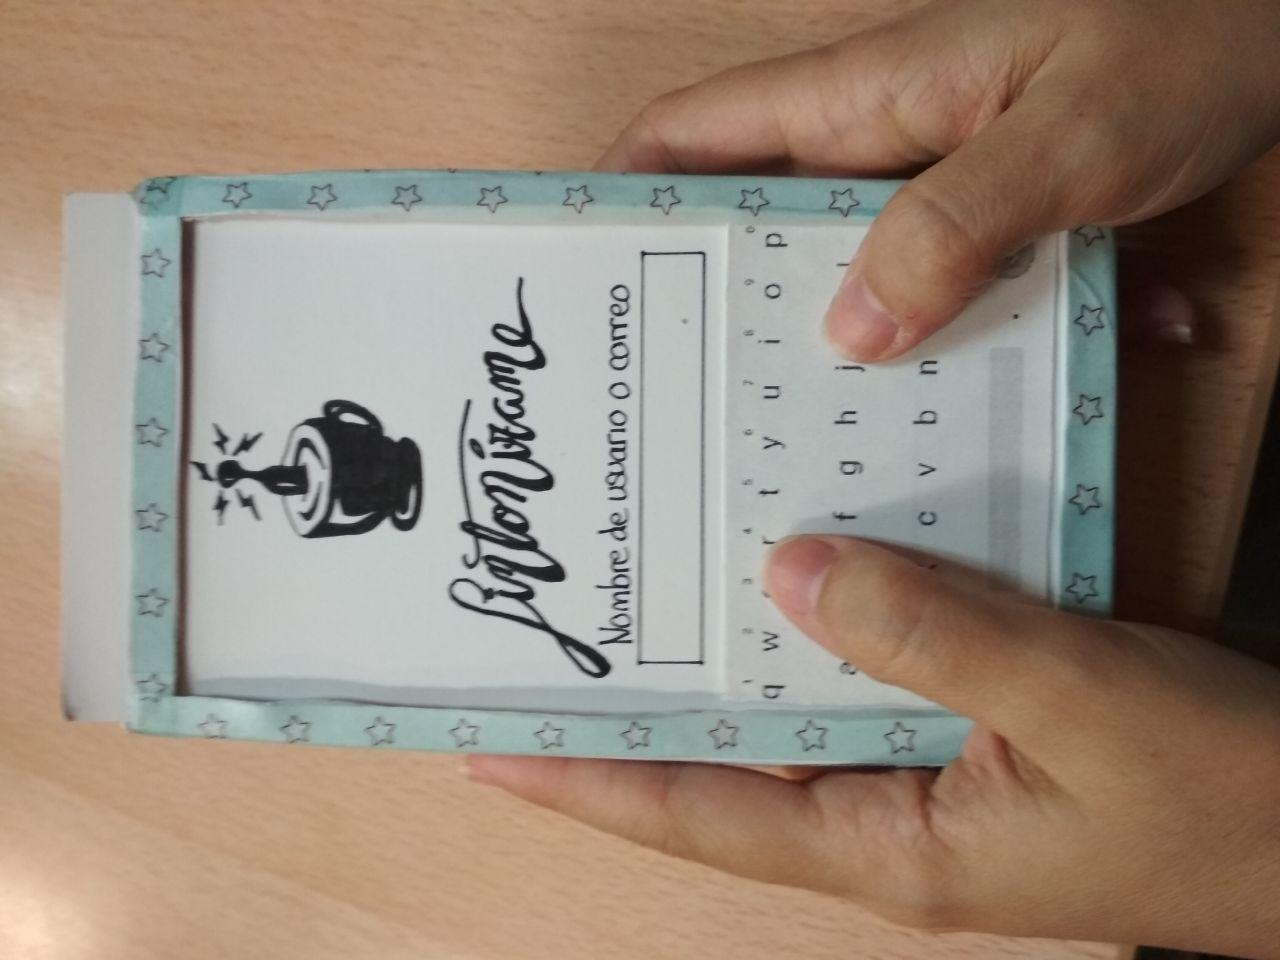
\includegraphics[height=0.4\columnwidth,angle=-90]{T1-3.jpg}
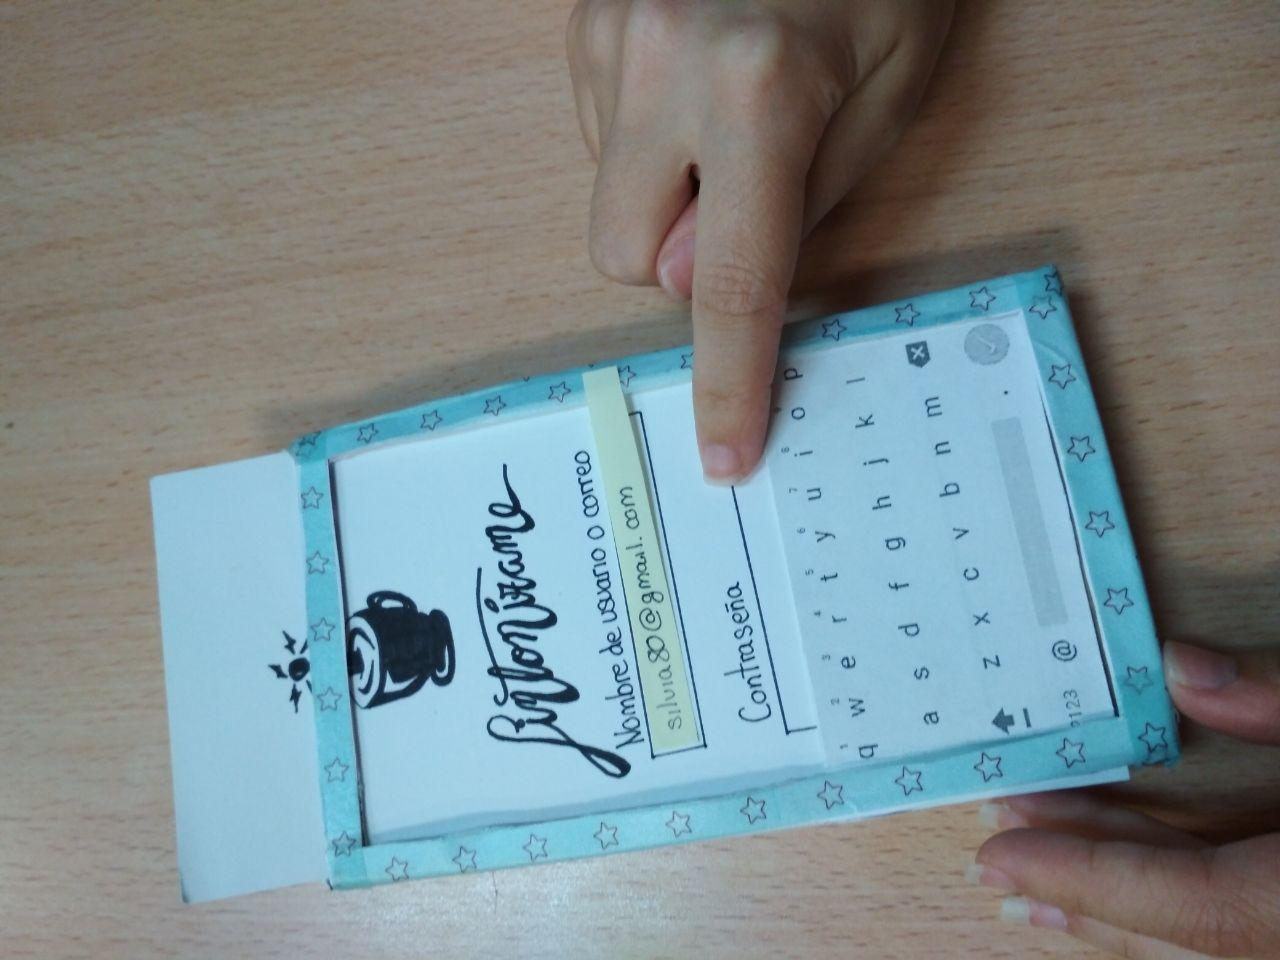
\includegraphics[height=0.4\columnwidth,angle=-90]{T1-4.jpg}
\caption{Introducir nombre de usuario}
Pulsando en las áreas de texto te sale un teclado qwerty para que puedas introducir los tus datos. Dando al tick del teclado salimos de este y podemos seguir desplazandonos por la vista introduciendo el resto de datos.
\label{fig:t1-3}
\end{figure}
\begin{figure}[H]
\centering
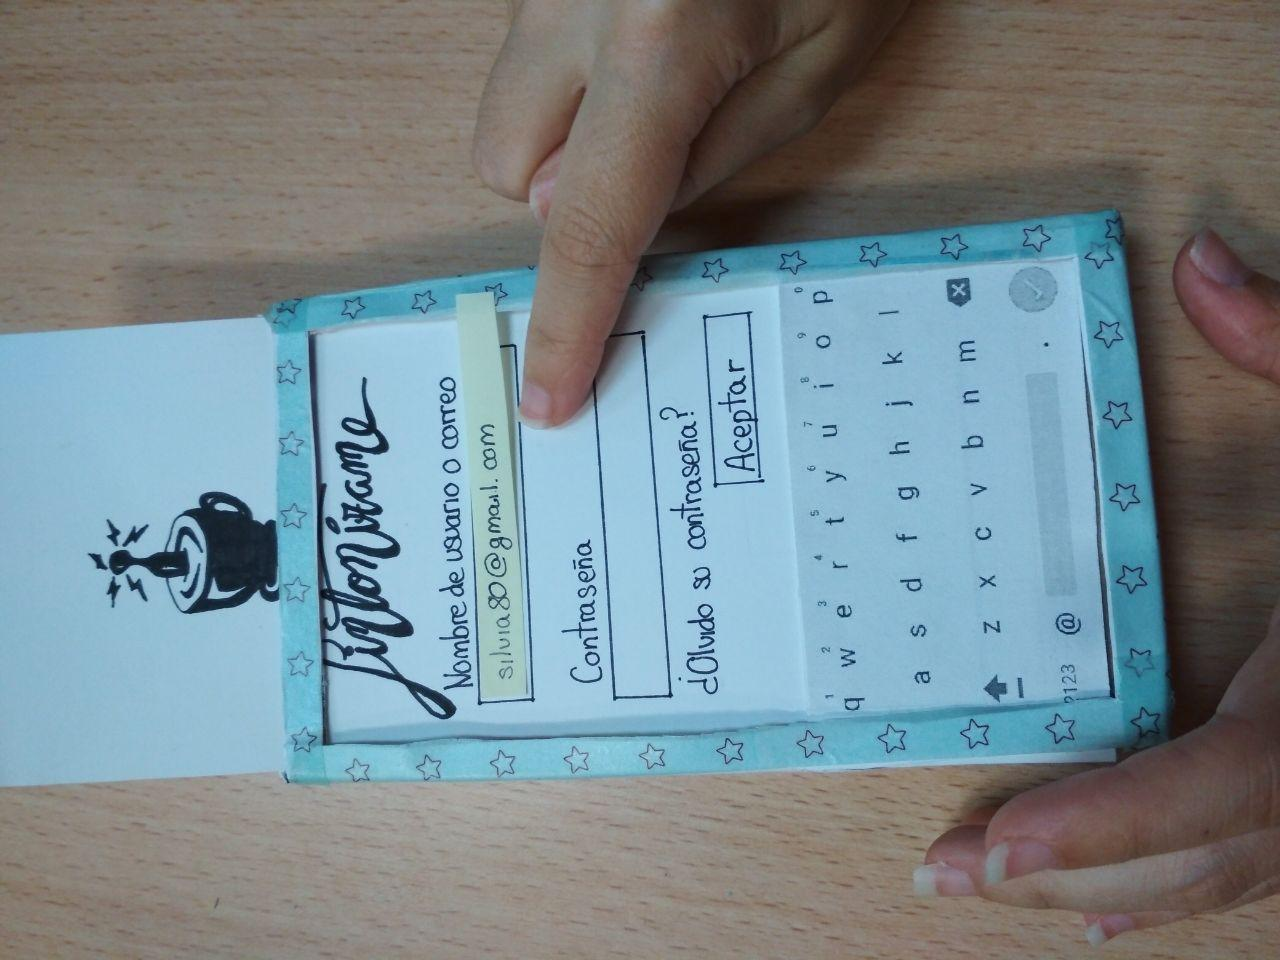
\includegraphics[height=0.4\columnwidth,angle=-90]{T1-5.jpg}
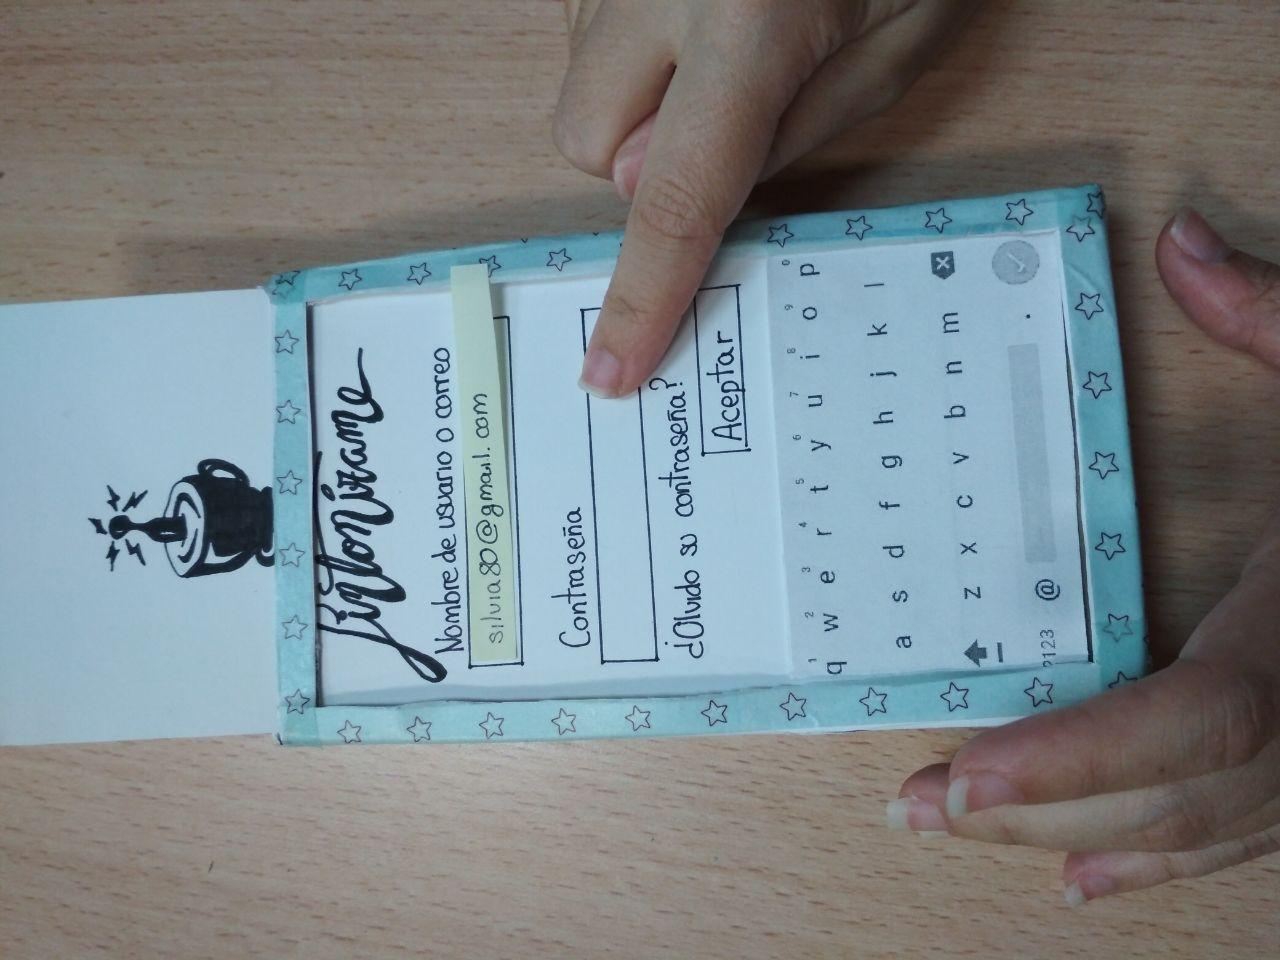
\includegraphics[height=0.4\columnwidth,angle=-90]{T1-6.jpg} 
\caption{Desplazar pantalla}
\label{fig:t1-5}
Arrastrando el dedo tenemos la posibilidad de desplazarnos por la pantalla.
\end{figure}
\begin{figure}[H]
\centering
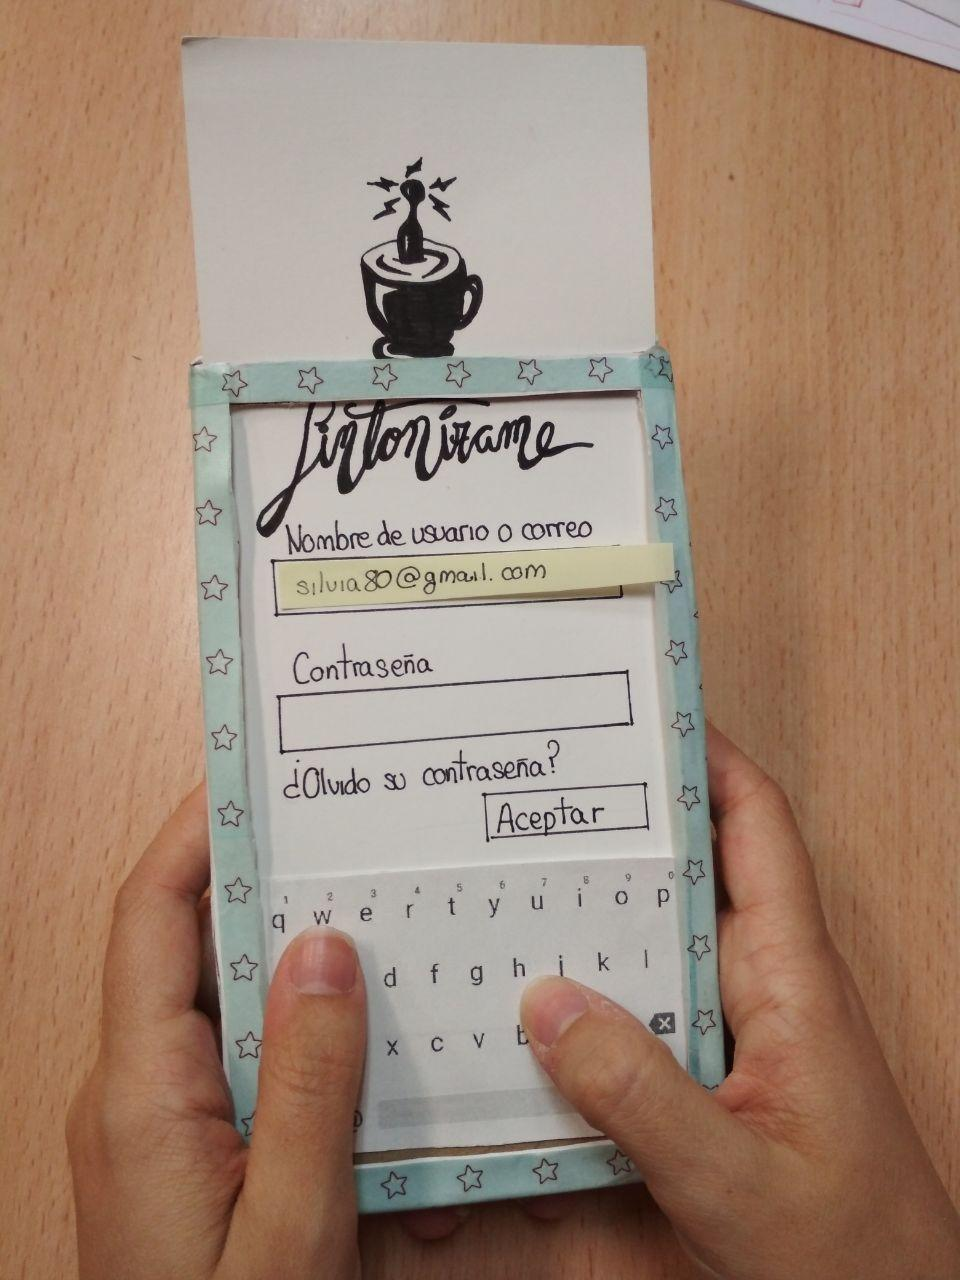
\includegraphics[width=0.4\columnwidth]{T1-7.jpg}
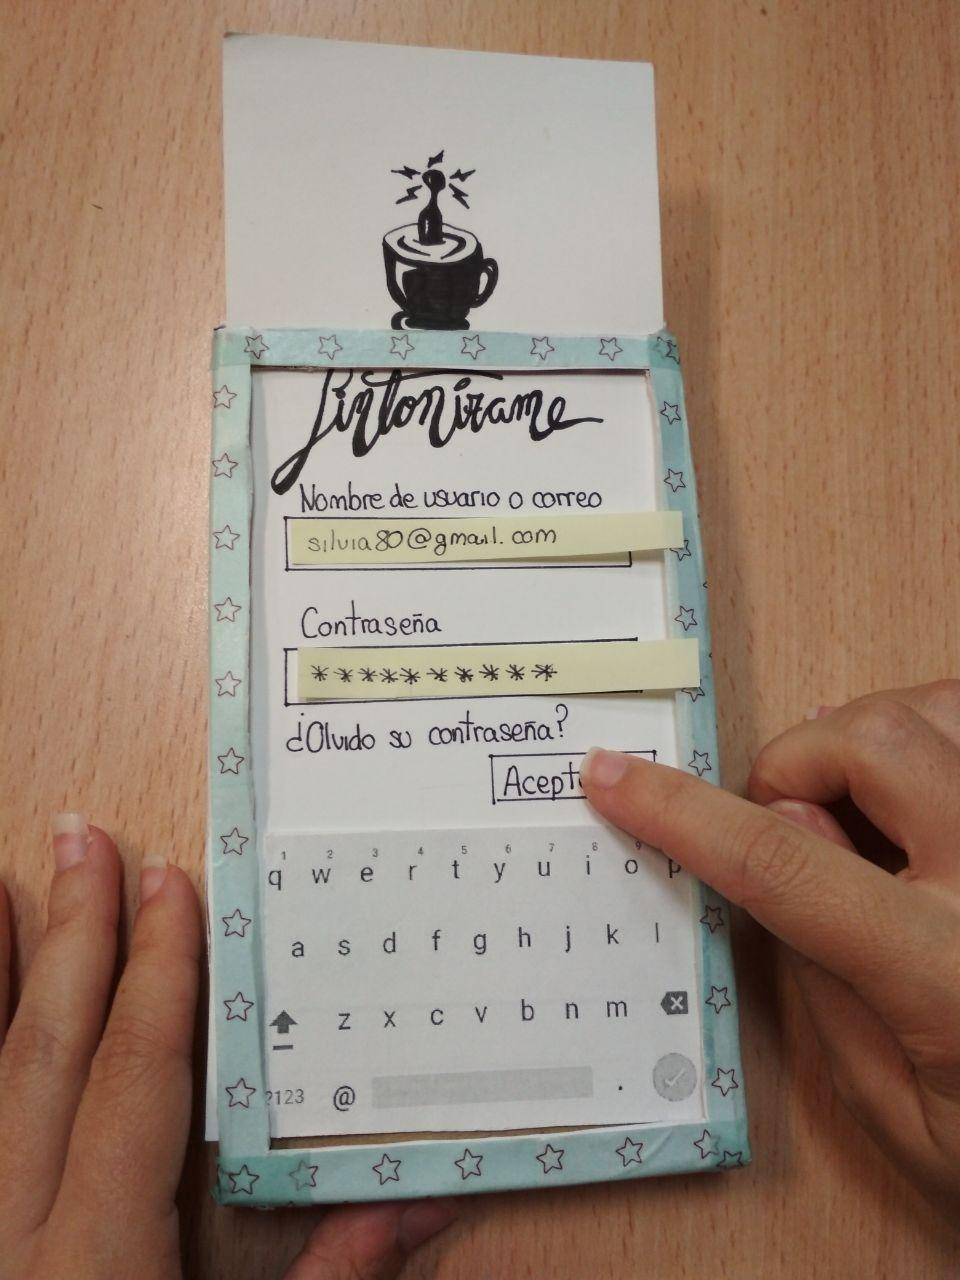
\includegraphics[width=0.4\columnwidth]{T1-8.jpg} 
\caption{Introducir contraseña}
Al igual que con el nombre de usuario se realizan los mismos pasos para introducir la contraseña. Para acceder definitivamente a la app tras haber introducido todos los datos necesarios tenemos un botón "Aceptar" que nos llevará a la primera vista de la aplicación.
\label{fig:t1-7}
\end{figure}
\end{center}

\subsection{Tarea 2}
\begin{center}
\begin{figure}[H]
\centering
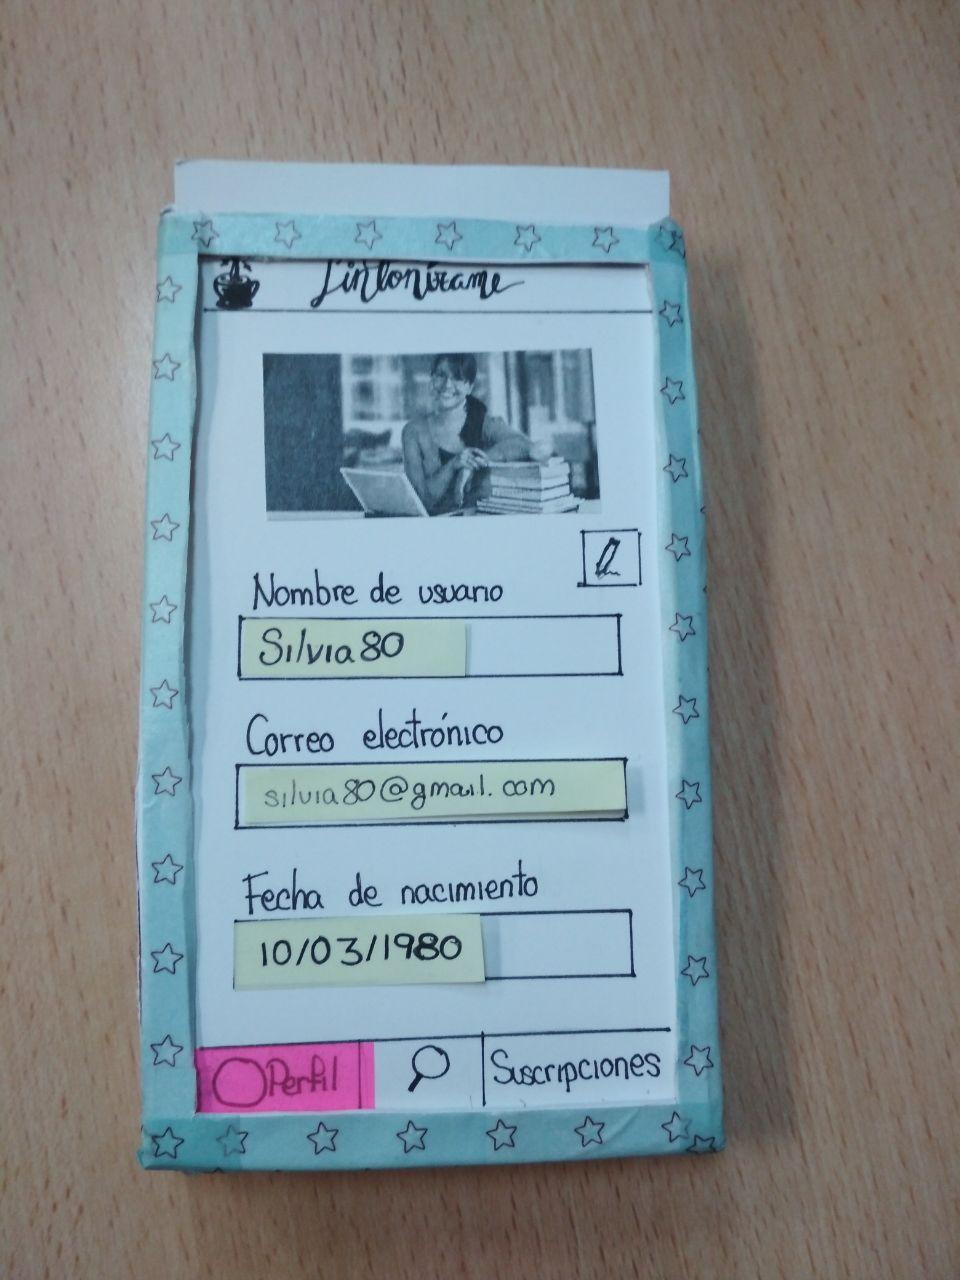
\includegraphics[width=0.4\columnwidth]{T2-1.jpg}
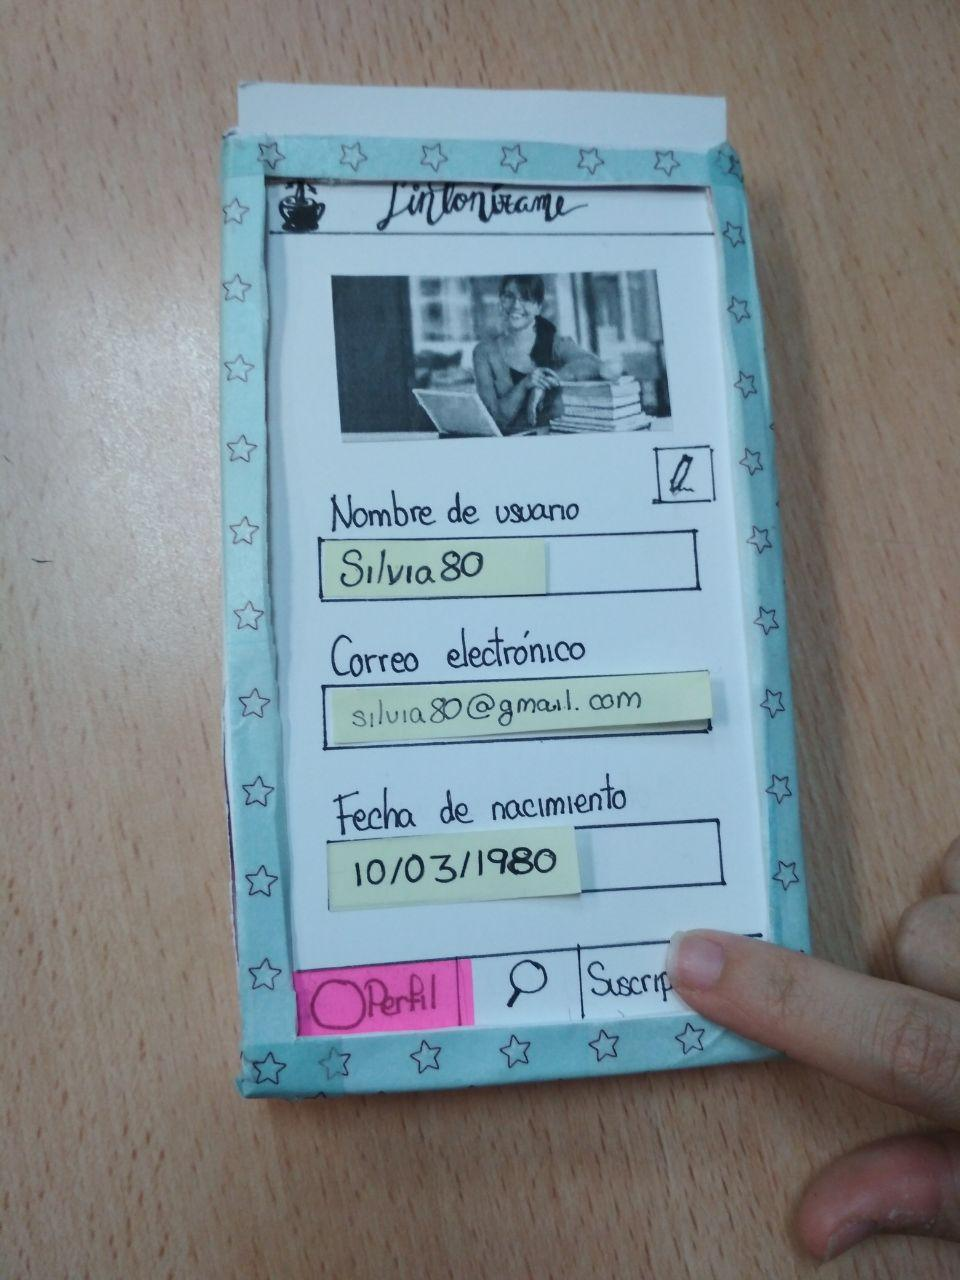
\includegraphics[width=0.4\columnwidth]{T2-2.jpg}
\caption{Acceder a mis suscripciones}
Nada más acceder a la aplicación nos encontramos con la pantalla de perfil, vemos una retroalimentación visual en el botón de perfil, para ello si queremos desplazarnos hacia nuestras suscripciones para ver si hay alguna nueva notificación basta simplemente con pulsar del botón de 'Suscripciones' que se pondrá en color rosa.
\label{fig:t2-1}
\end{figure}
\begin{figure}[H]
\centering
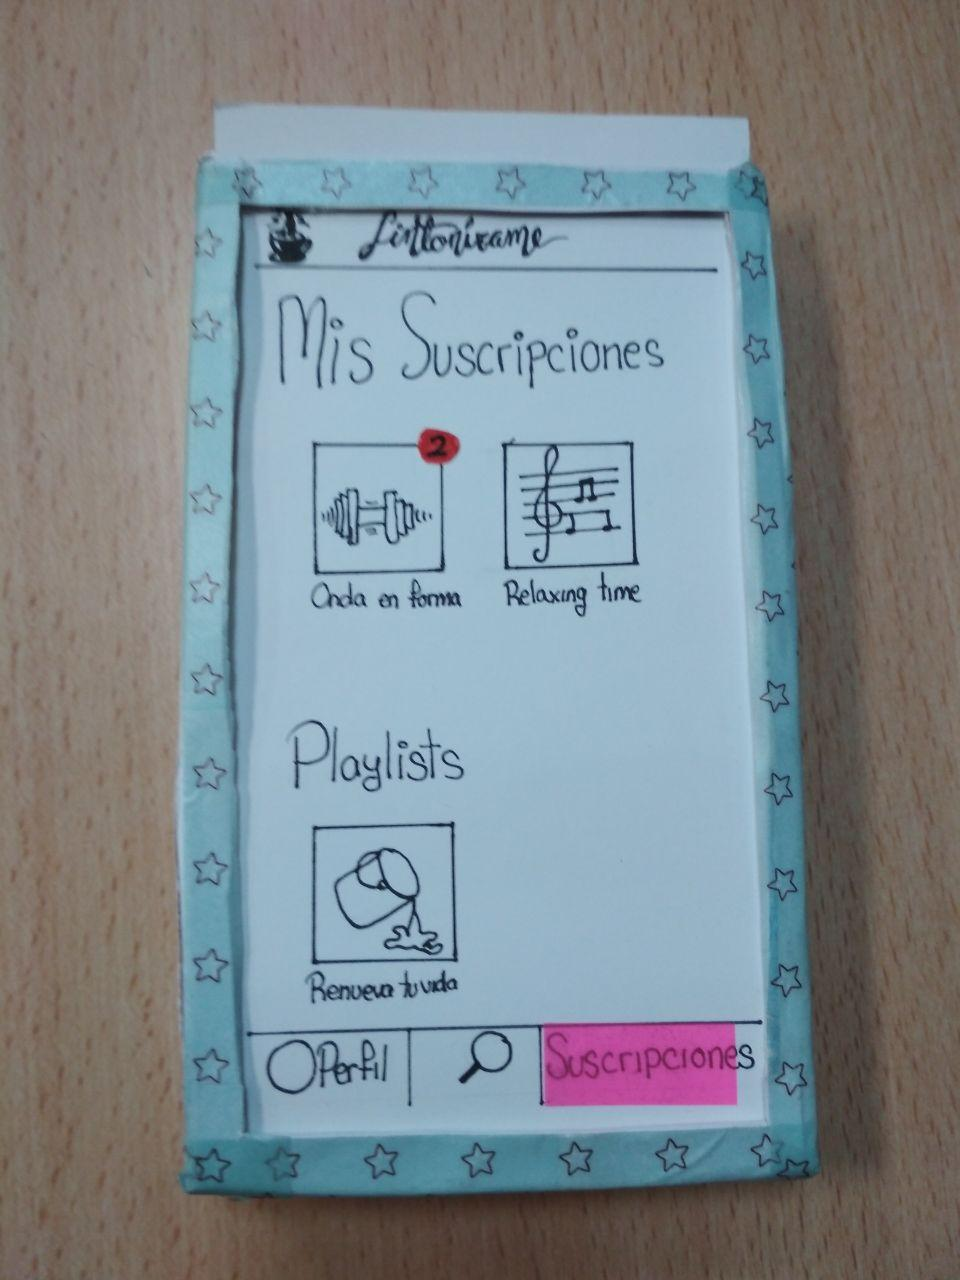
\includegraphics[width=0.4\columnwidth]{T2-3.jpg}
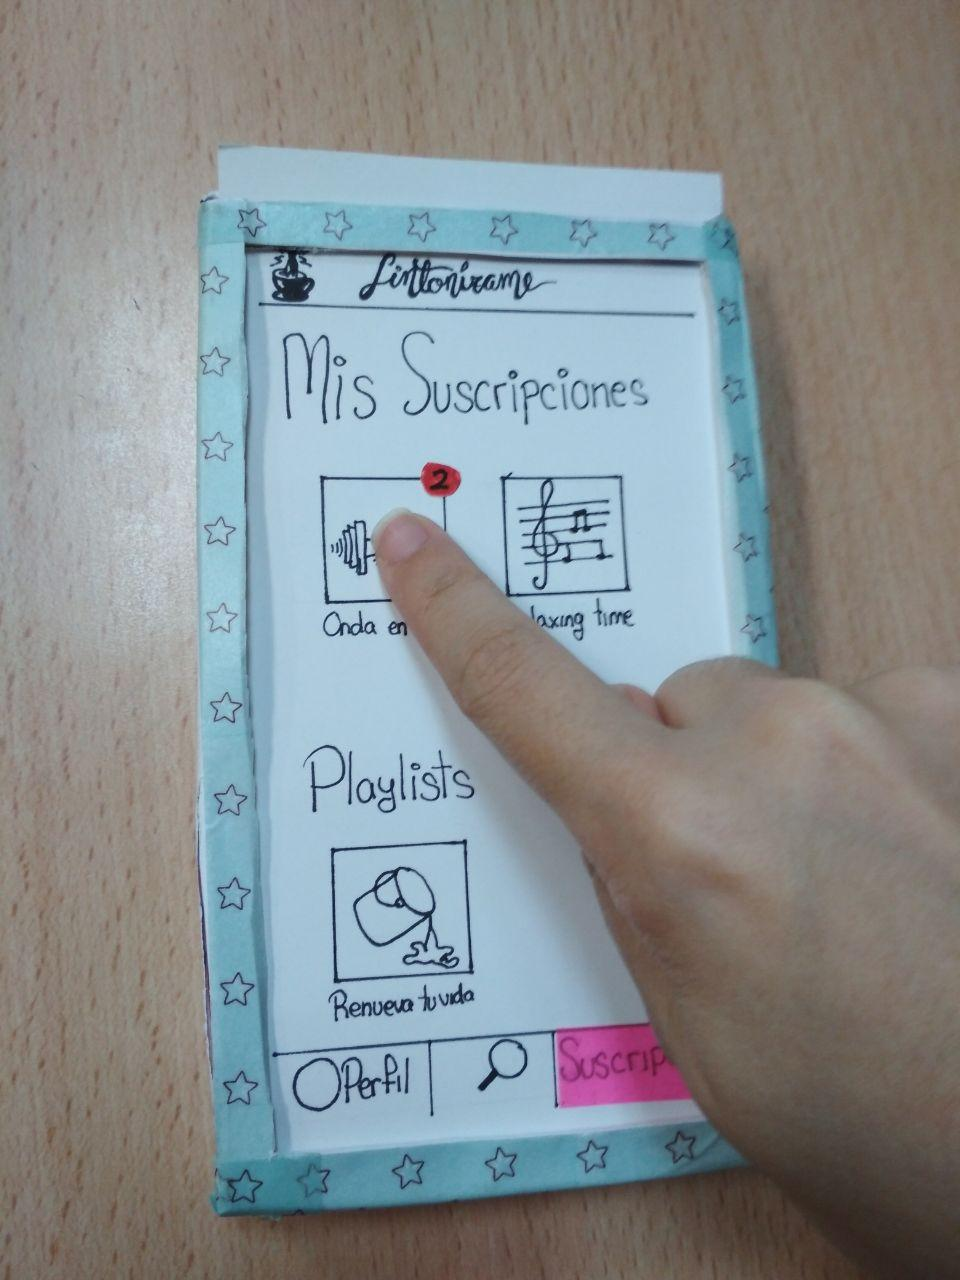
\includegraphics[width=0.4\columnwidth]{T2-4.jpg}
\caption{Acceder a nuevos podcasts}
Los canales que tengan algún nuevo podcast se mostraran con un pop-up rojo sobre ellos indicando el número de nuevas pistas para escuchar. Si accedemos al canal nos mostrará una lista de los podcasts/pistas.
\label{fig:t2-3}
\end{figure}
\begin{figure}[H]
\centering
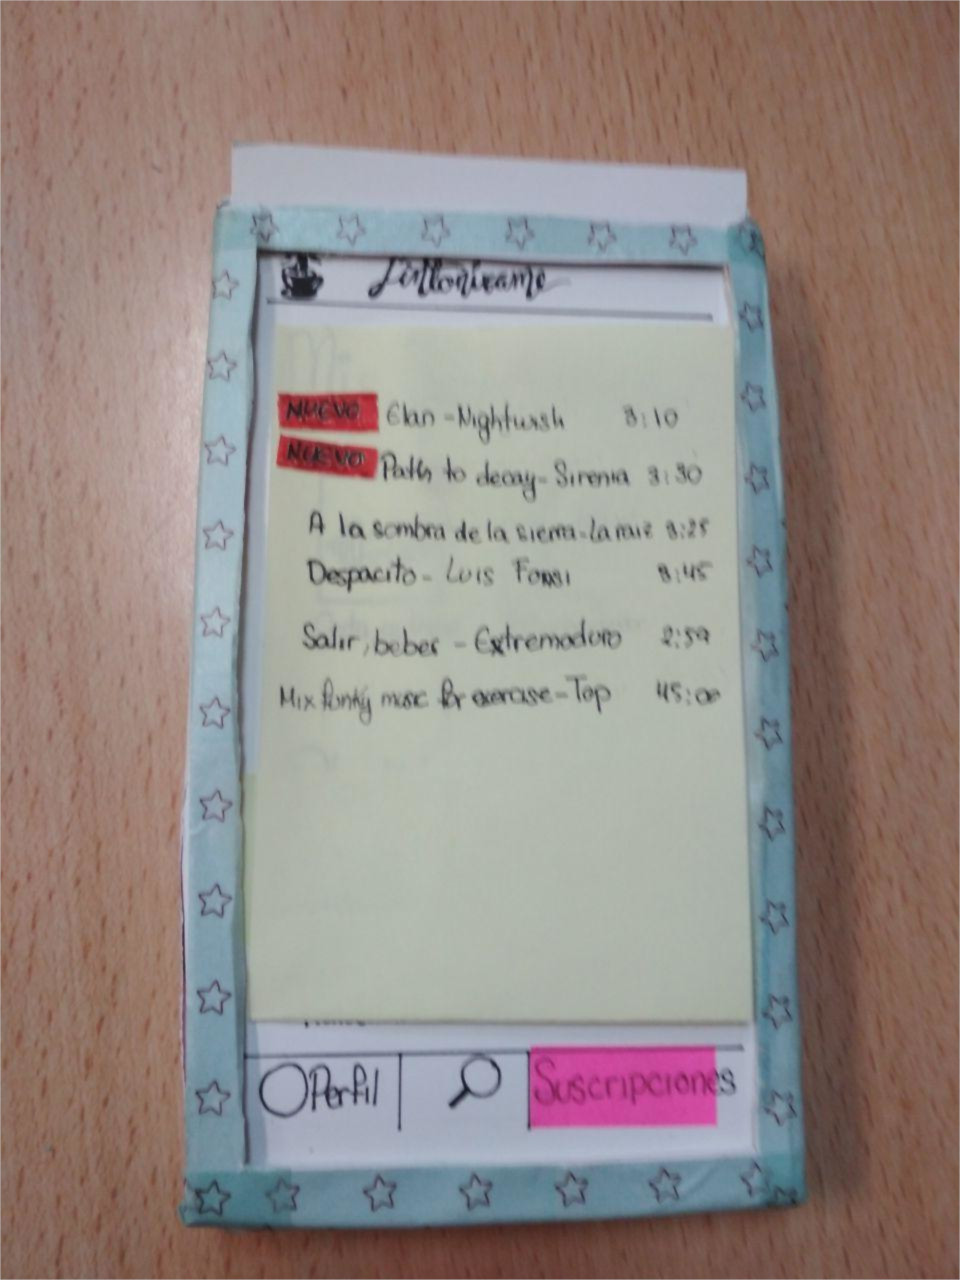
\includegraphics[width=0.4\columnwidth]{T2-5.jpg}
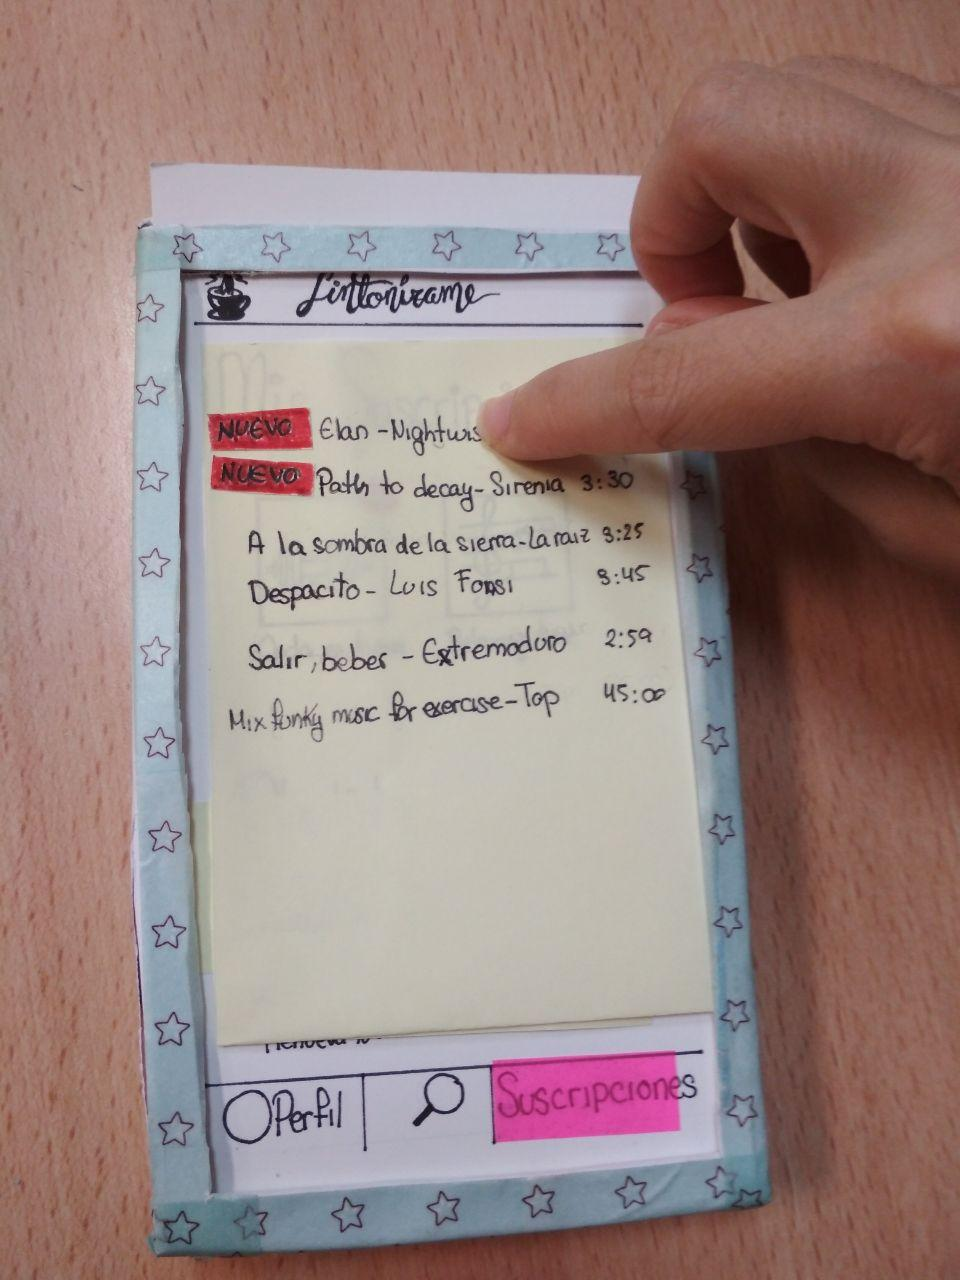
\includegraphics[width=0.4\columnwidth]{T2-6.jpg}
\caption{Ver lista de nuevos podcasts}
\label{fig:t2-5}
Los podcasts o pistas que sean nuevas estarán marcadas con una etiqueta de 'nuevo' y podremos acceder a la que queremos simplemente pulsando sobre una de ellas.
\end{figure}
\begin{figure}[H]
\centering
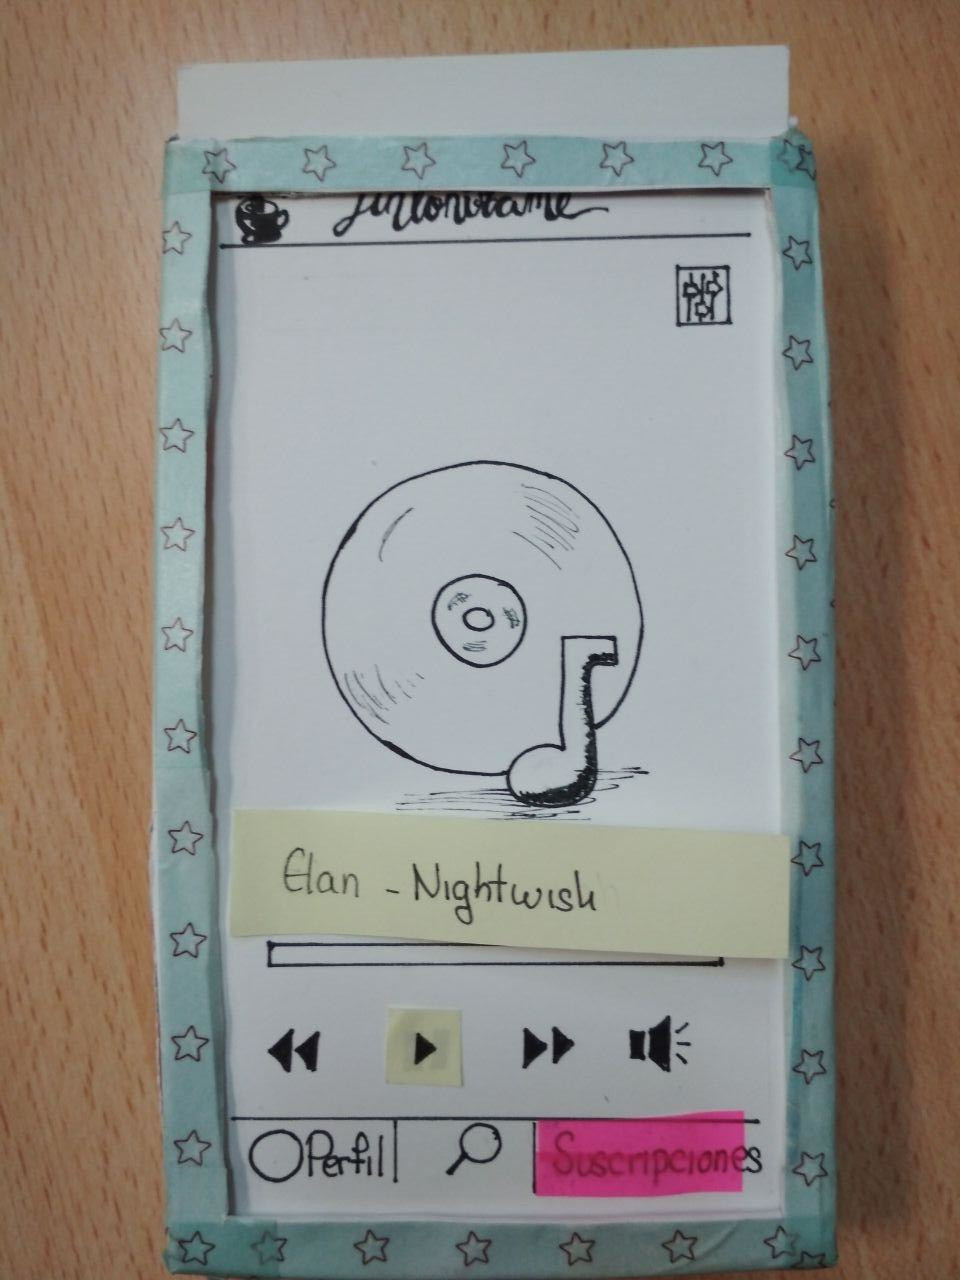
\includegraphics[width=0.4\columnwidth]{T2-6b.jpg}
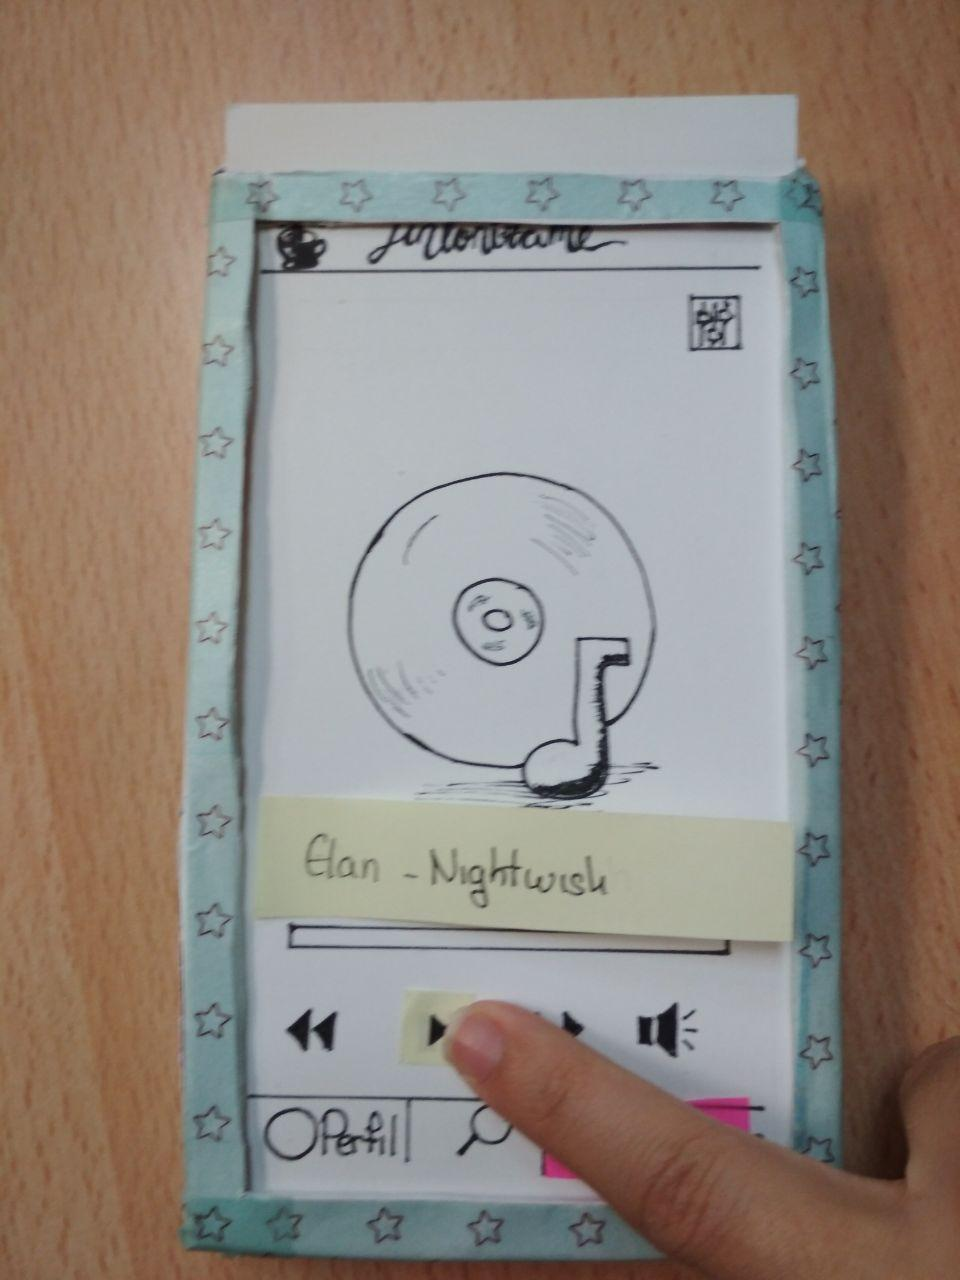
\includegraphics[width=0.4\columnwidth]{T2-6c.jpg}
\caption{Escuchar un podcast nuevo}
Tras seleccionar una pista la aplicación permitirá escucharla simplemente dándole al botón de play para que comience la reproducción y el botón de pause para detenerla.
\label{fig:t2-7}
\end{figure}
\begin{figure}[H]
\centering
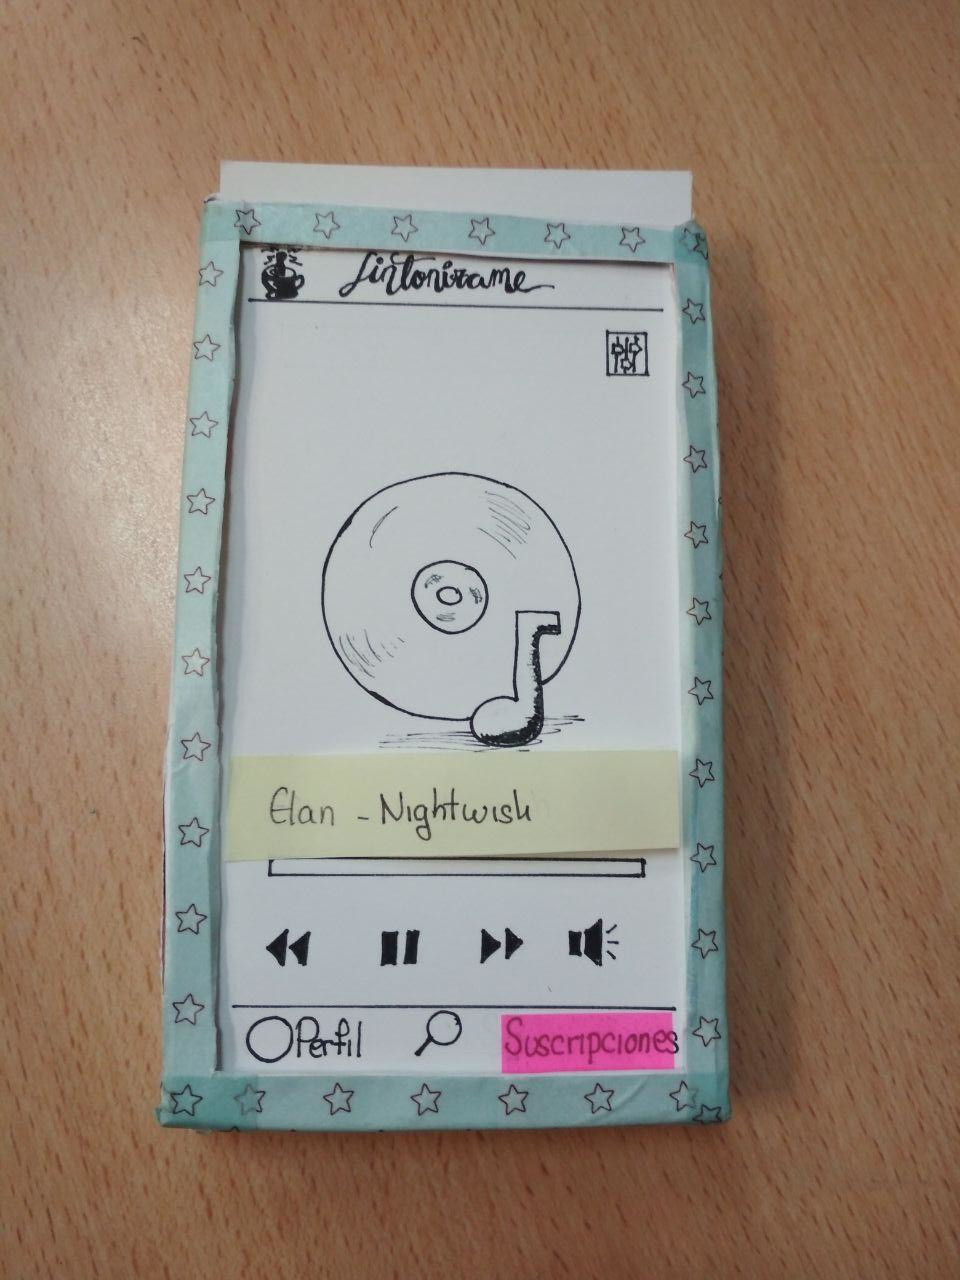
\includegraphics[width=0.4\columnwidth]{T2-7.jpg}
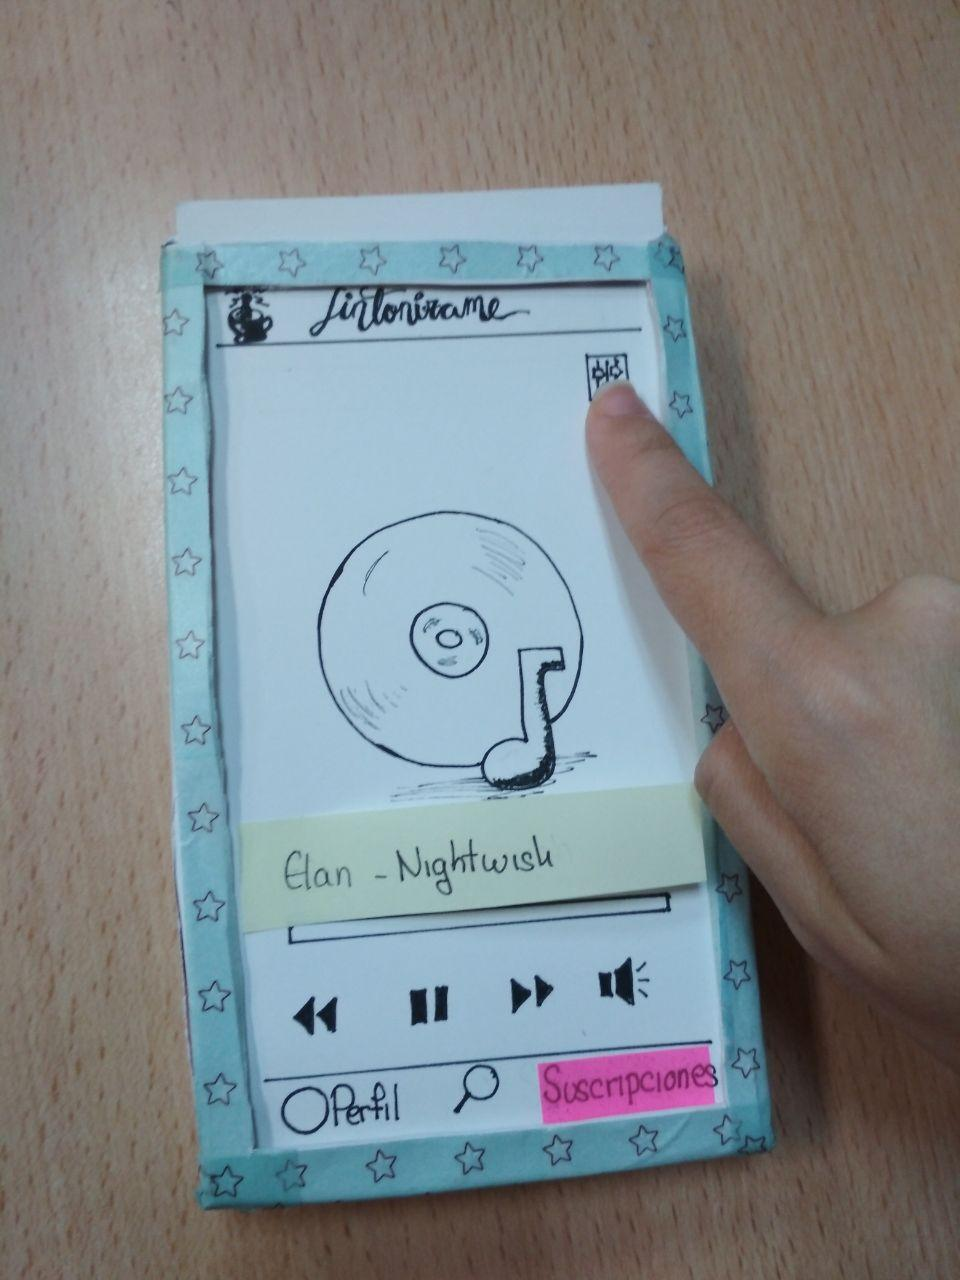
\includegraphics[width=0.4\columnwidth]{T2-8.jpg}
\caption{Acceder a ajustes de sonido}
Podemos acceder a los ajustes de sonido simplemente pulsando en el botón de ecualizador, este se mostrará en rosa y nos mostrará las diferentes opciones.
\label{fig:t2-9}
\end{figure}
\begin{figure}[H]
\centering
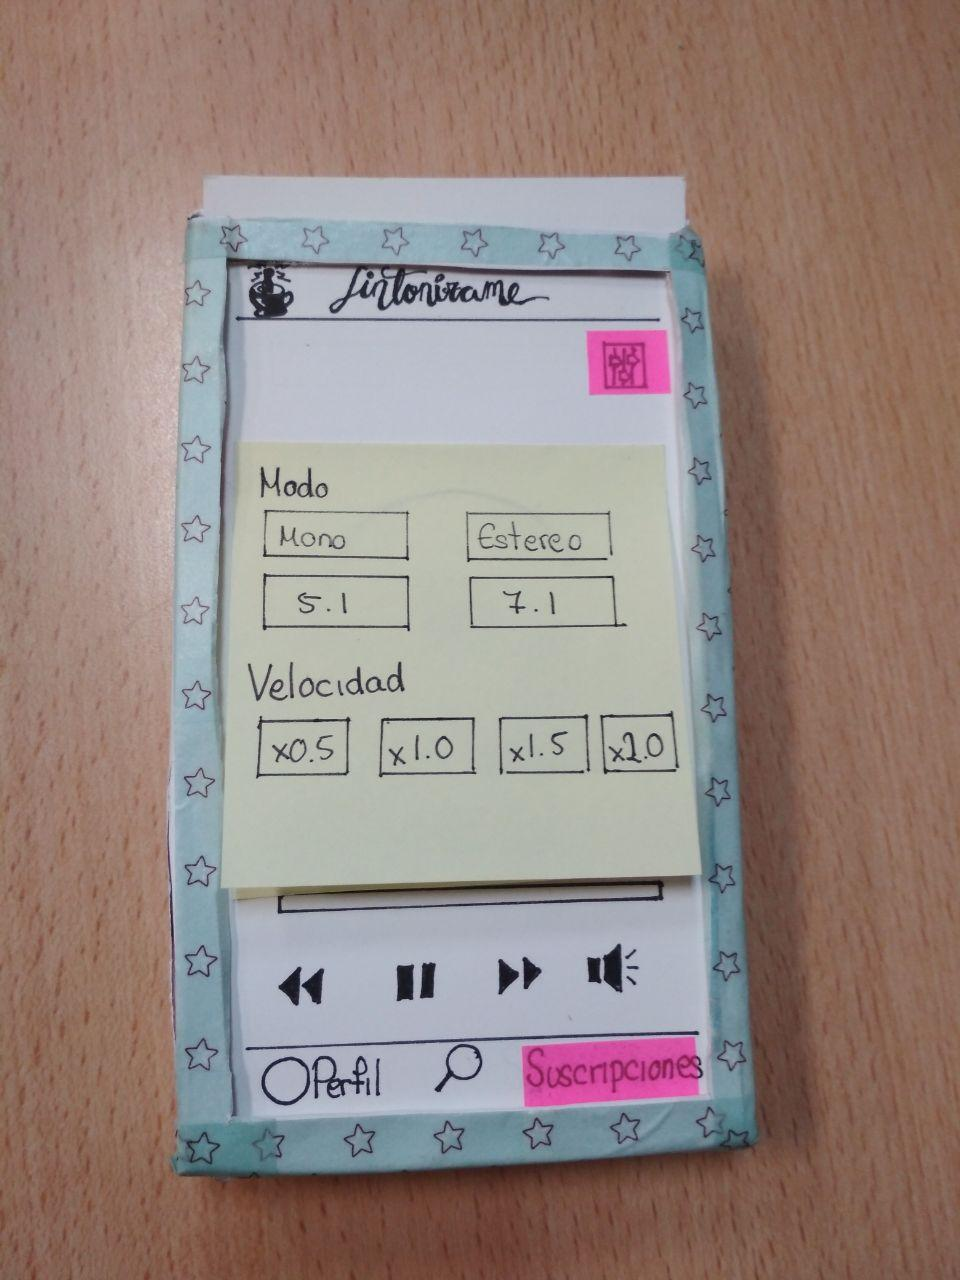
\includegraphics[width=0.4\columnwidth]{T2-9.jpg}
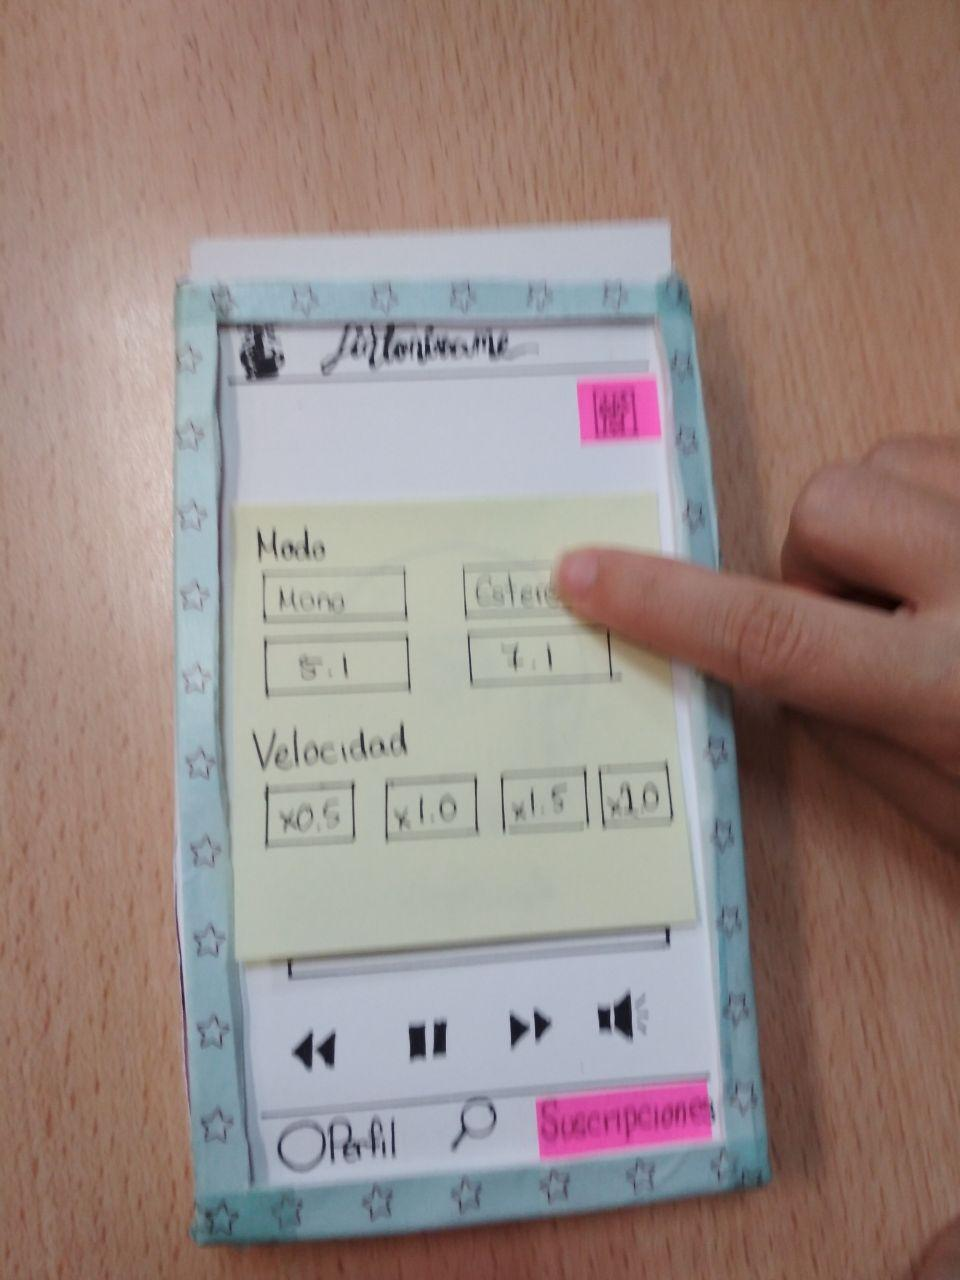
\includegraphics[width=0.4\columnwidth]{T2-10.jpg}
\caption{Cambiar a modo estéreo}
Dentro de los ajustes podremos seleccionar el modo de sonido e incluso la velocidad de reproducción.
\label{fig:t2-11}
\end{figure}
\begin{figure}[H]
\centering
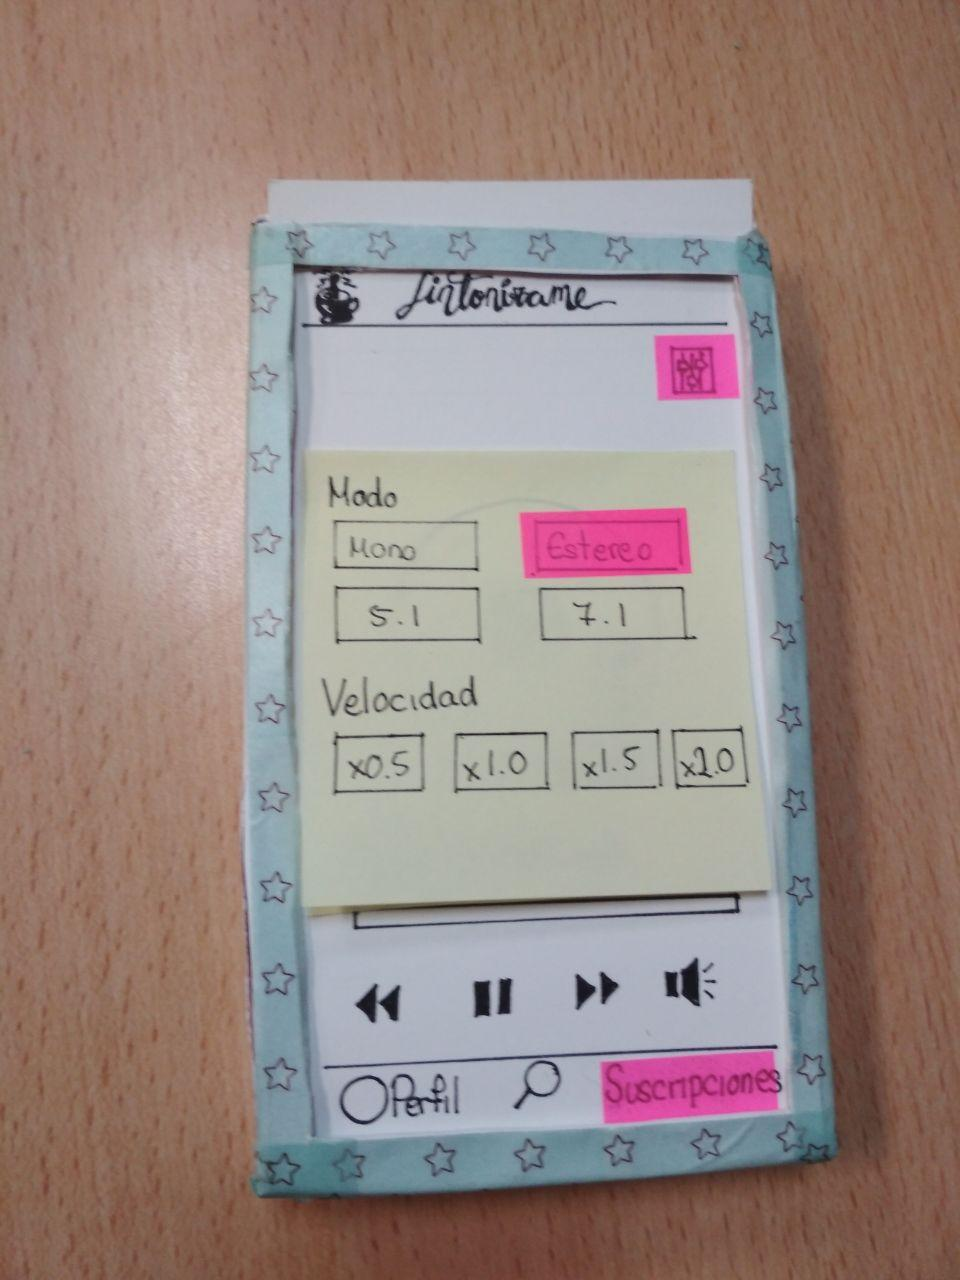
\includegraphics[width=0.4\columnwidth]{T2-11.jpg}
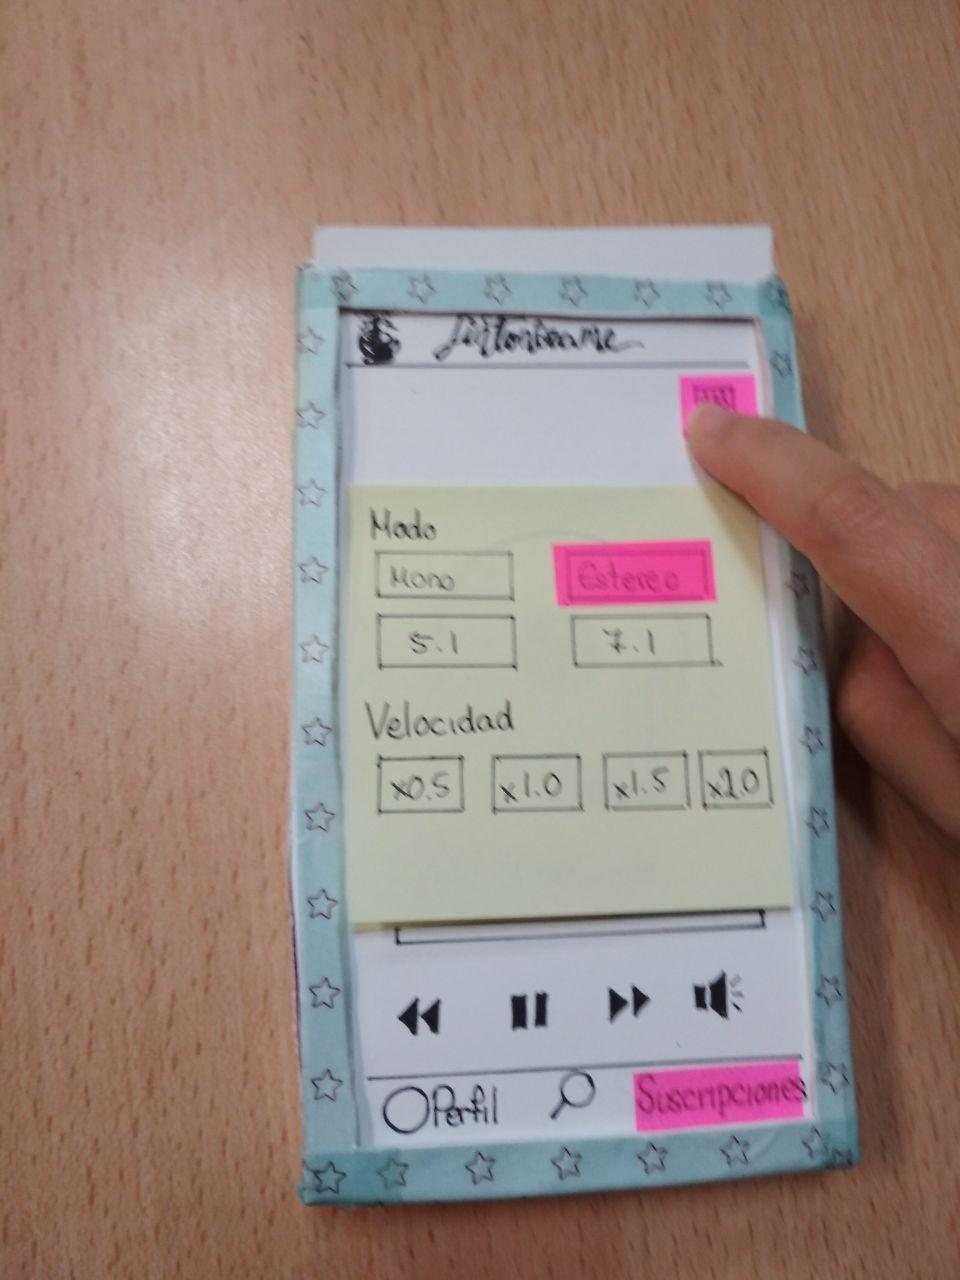
\includegraphics[width=0.4\columnwidth]{T2-12.jpg}
\caption{Cerrar ajustes de sonido}
Para salir de los ajustes basta con volver a pulsar el botón del ecualizador para que este se deseleccione y muestre de nuevo la vista de reproducción.
\label{fig:t2-13}
\end{figure}
\begin{figure}[H]
\centering
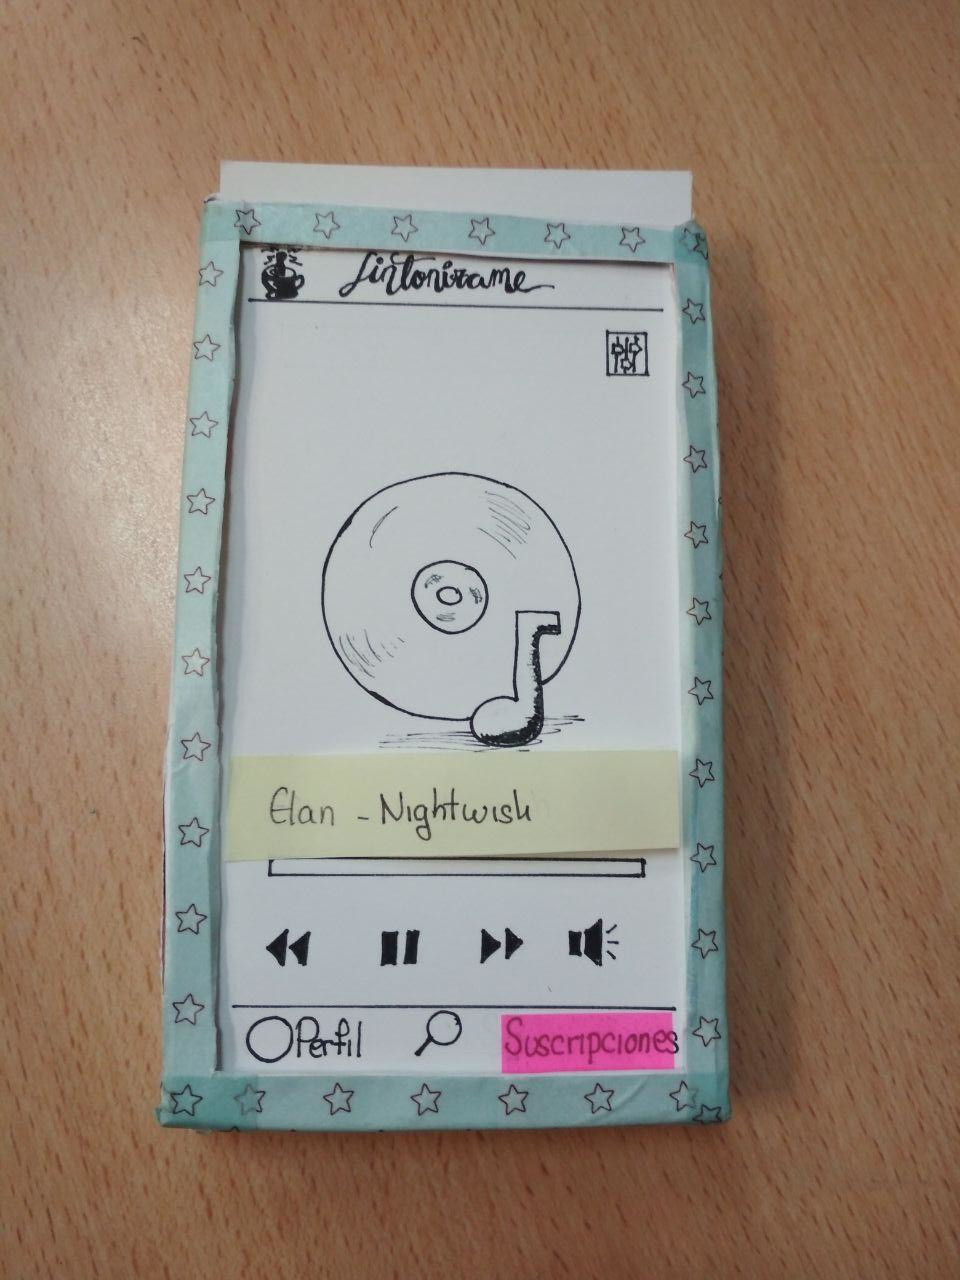
\includegraphics[width=0.4\columnwidth]{T2-7.jpg}
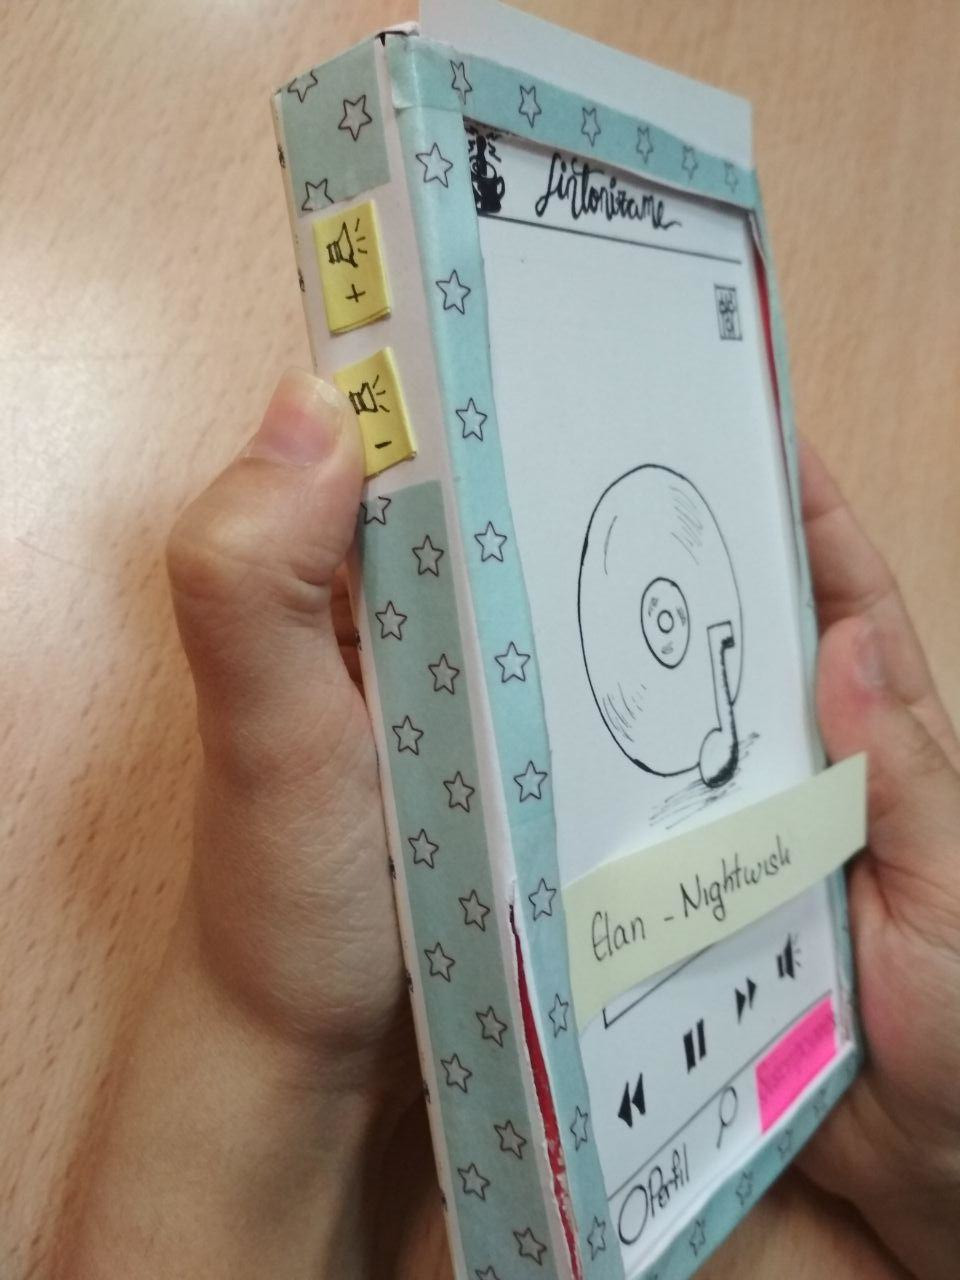
\includegraphics[width=0.4\columnwidth]{T2-13.jpg}
\caption{Bajar volumen}
Podemos subir y bajar el volumen de la pista pulsando los dos botones que hay al lateral del smartphone.
\label{fig:t2-15}
\end{figure}
\begin{figure}[H]
\centering
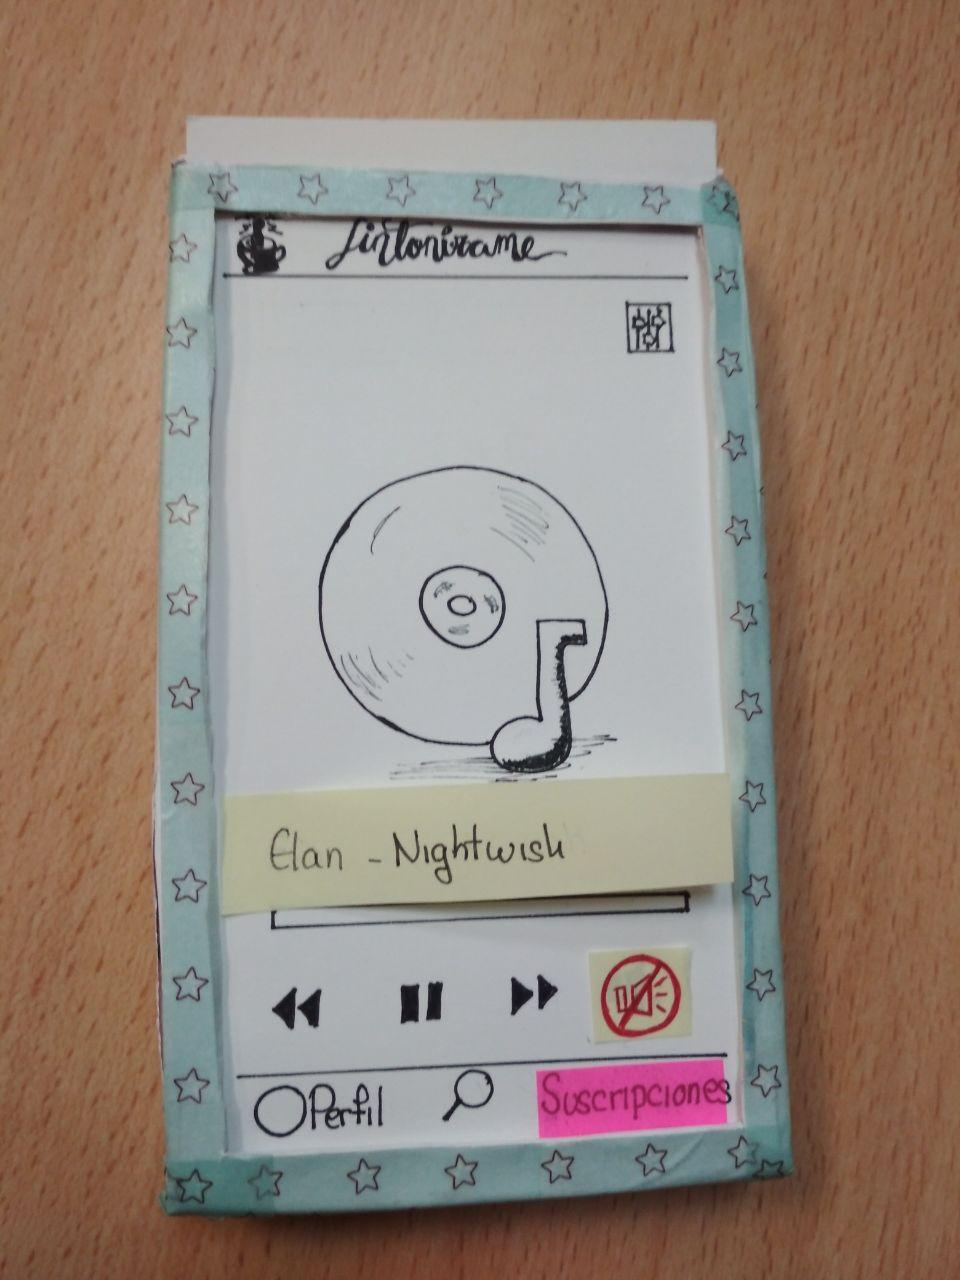
\includegraphics[width=0.4\columnwidth]{T2-14.jpg}
\caption{Silenciar}
\label{fig:t2-17}
Realizando el paso anterior y bajando el volumen podemos llenar a silenciar la pista.
\end{figure}
\end{center}

\subsection{Tarea 3}
\begin{center}
\begin{figure}[H]
\centering
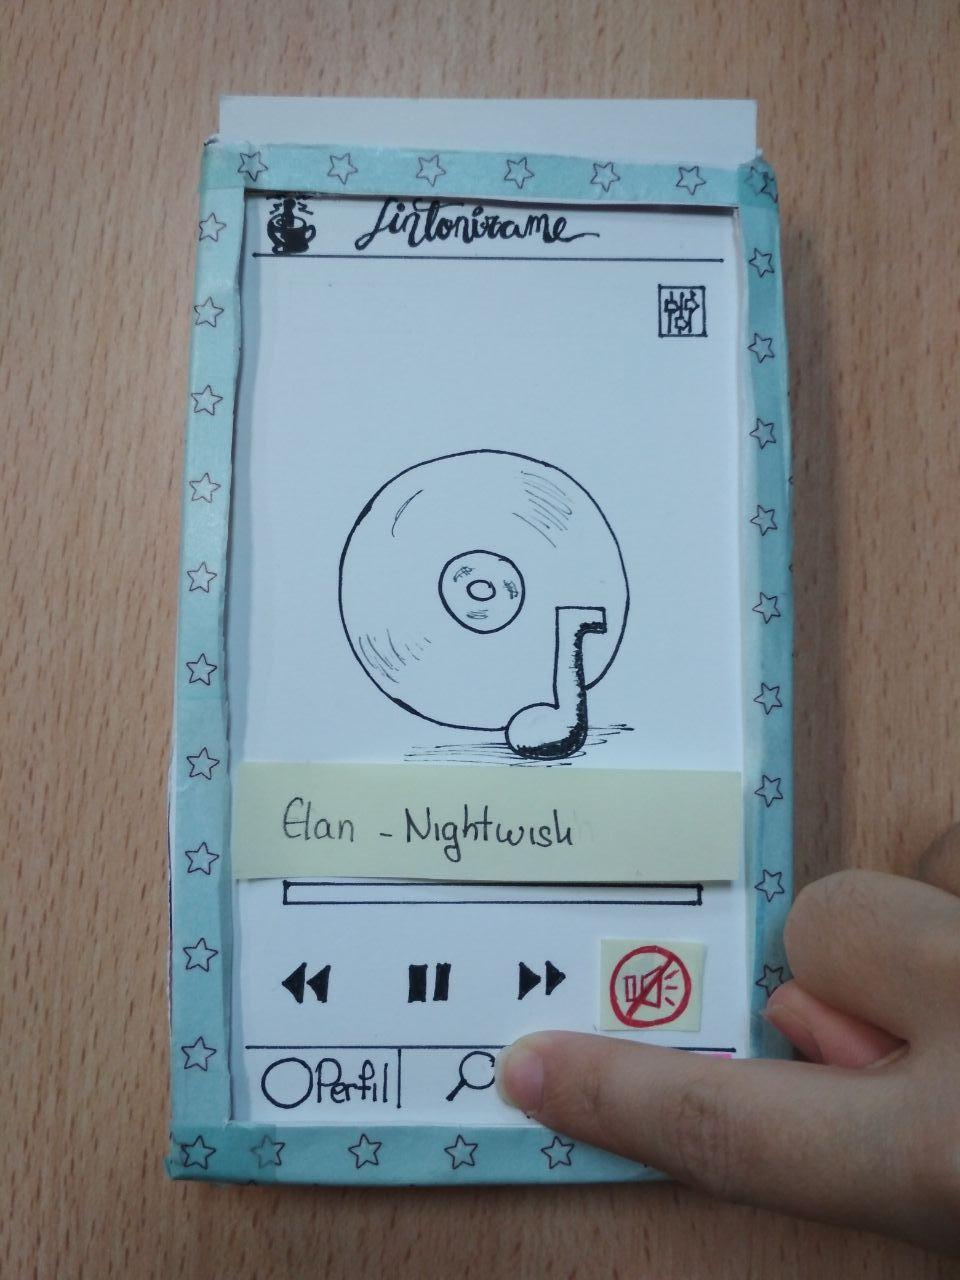
\includegraphics[width=0.4\columnwidth]{T3-19.jpg}
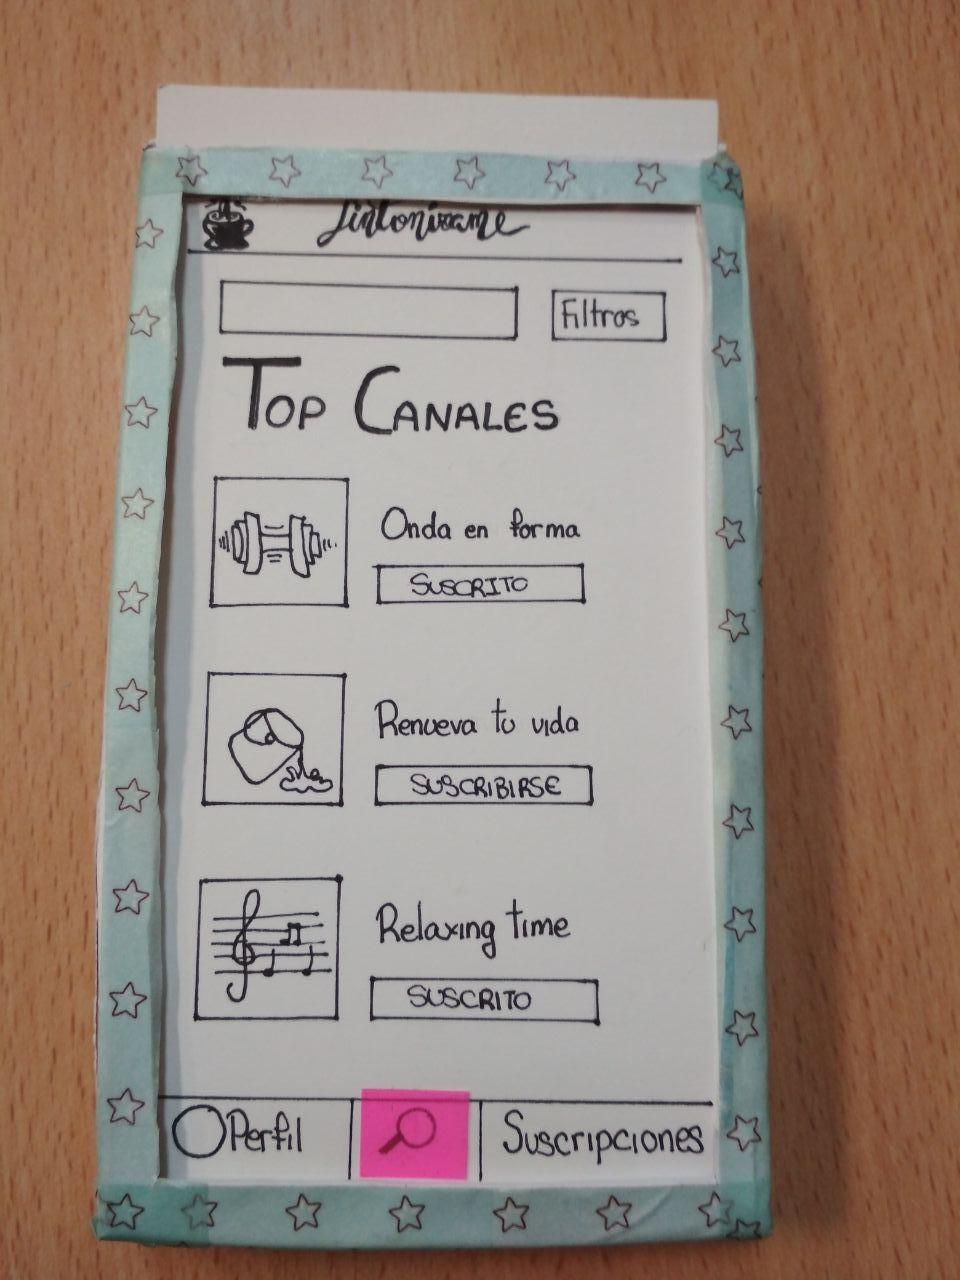
\includegraphics[width=0.4\columnwidth]{T3-18.jpg}
\caption{Acceder al buscador}
Si pulsamos en la lupa nos mostrará el buscador de la aplicación junto a un top de los canales a los que más usuarios hay suscritos.
\label{fig:t3-1}
\end{figure}
\begin{figure}[H]
\centering
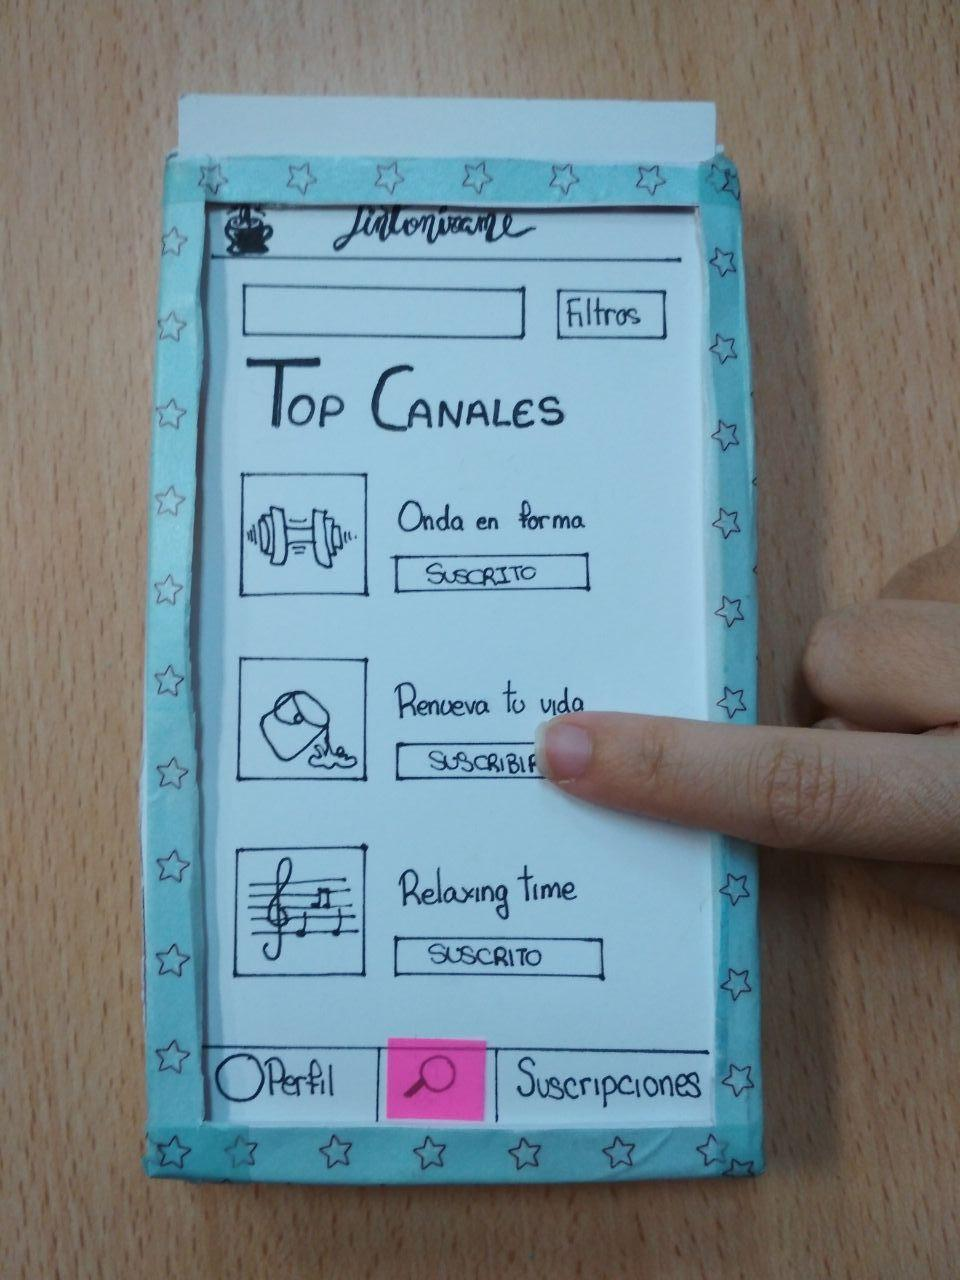
\includegraphics[width=0.4\columnwidth]{T3-17.jpg}
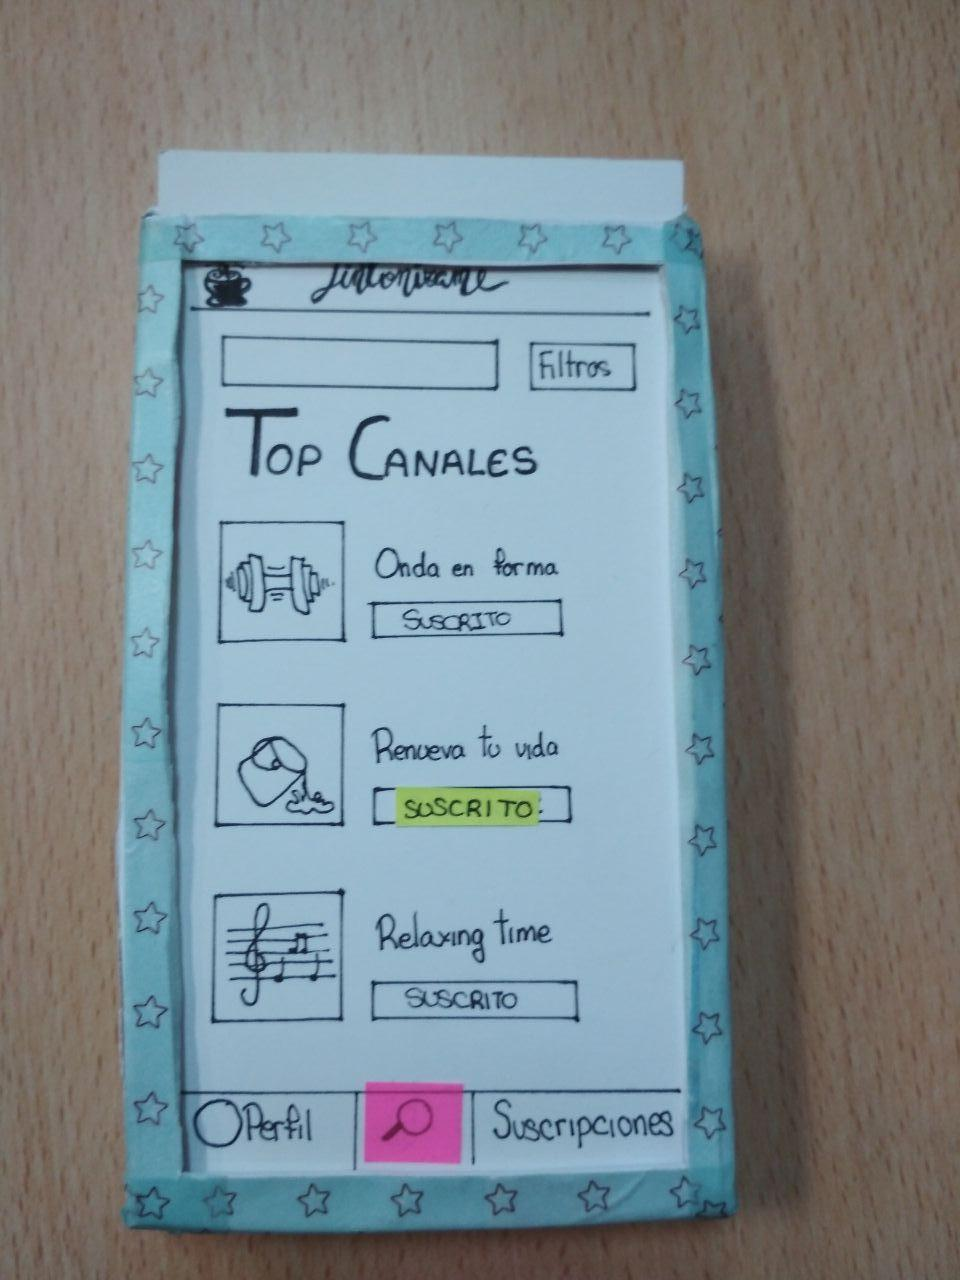
\includegraphics[width=0.4\columnwidth]{T3-16.jpg}
\caption{Suscribirse a decoración}
\label{fig:t3-3}
Para suscribirse a un canal como es el de decoración es tan fácil como pulsar el botón de suscribirse que se encuentra en el lateral derecho del logo/imagen del canal. Una vez realizado se te mostrará como suscrito.
\end{figure}
\begin{figure}[H]
\centering
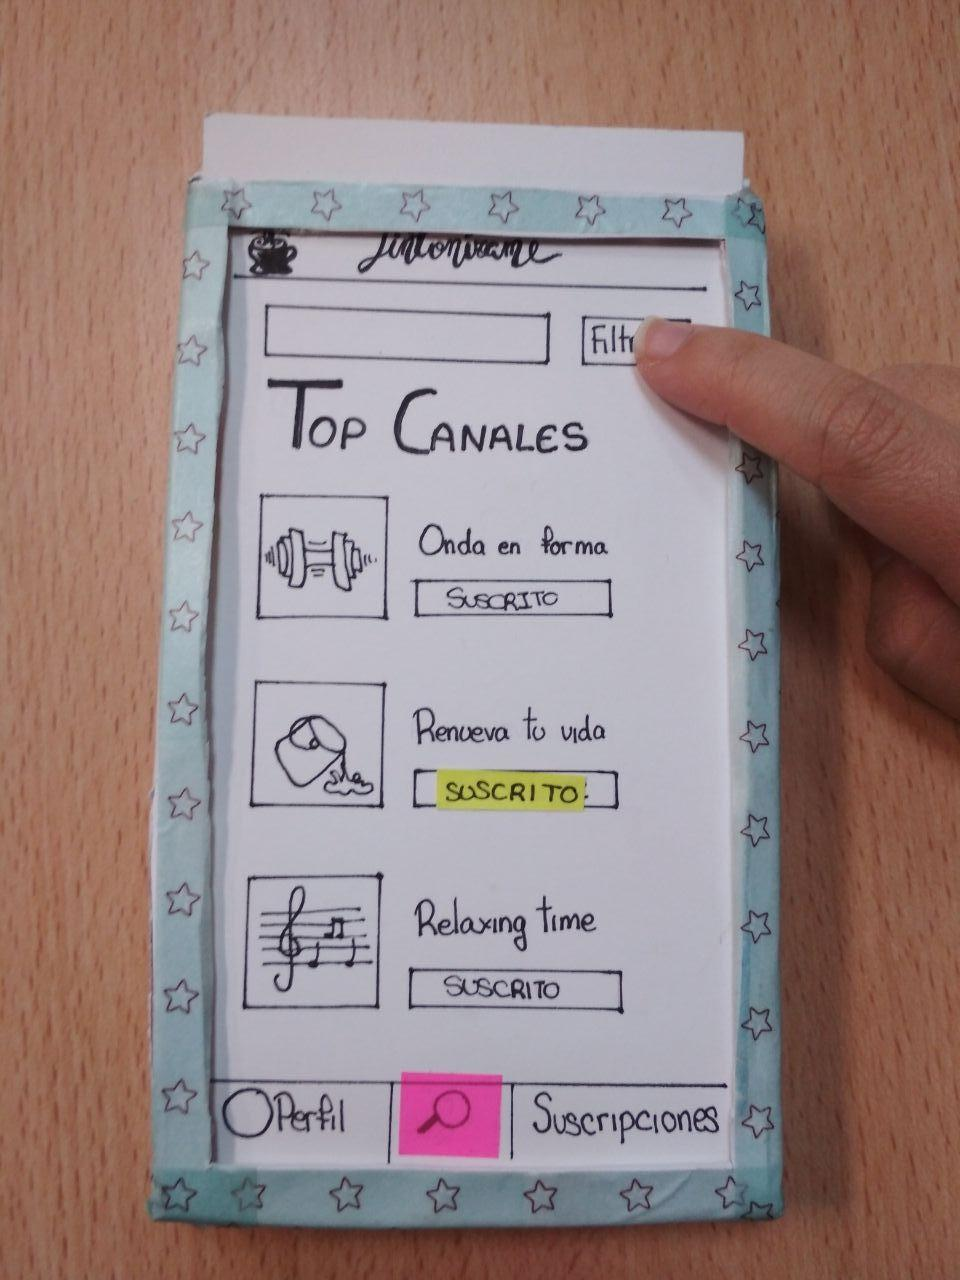
\includegraphics[width=0.4\columnwidth]{T3-11.jpg}
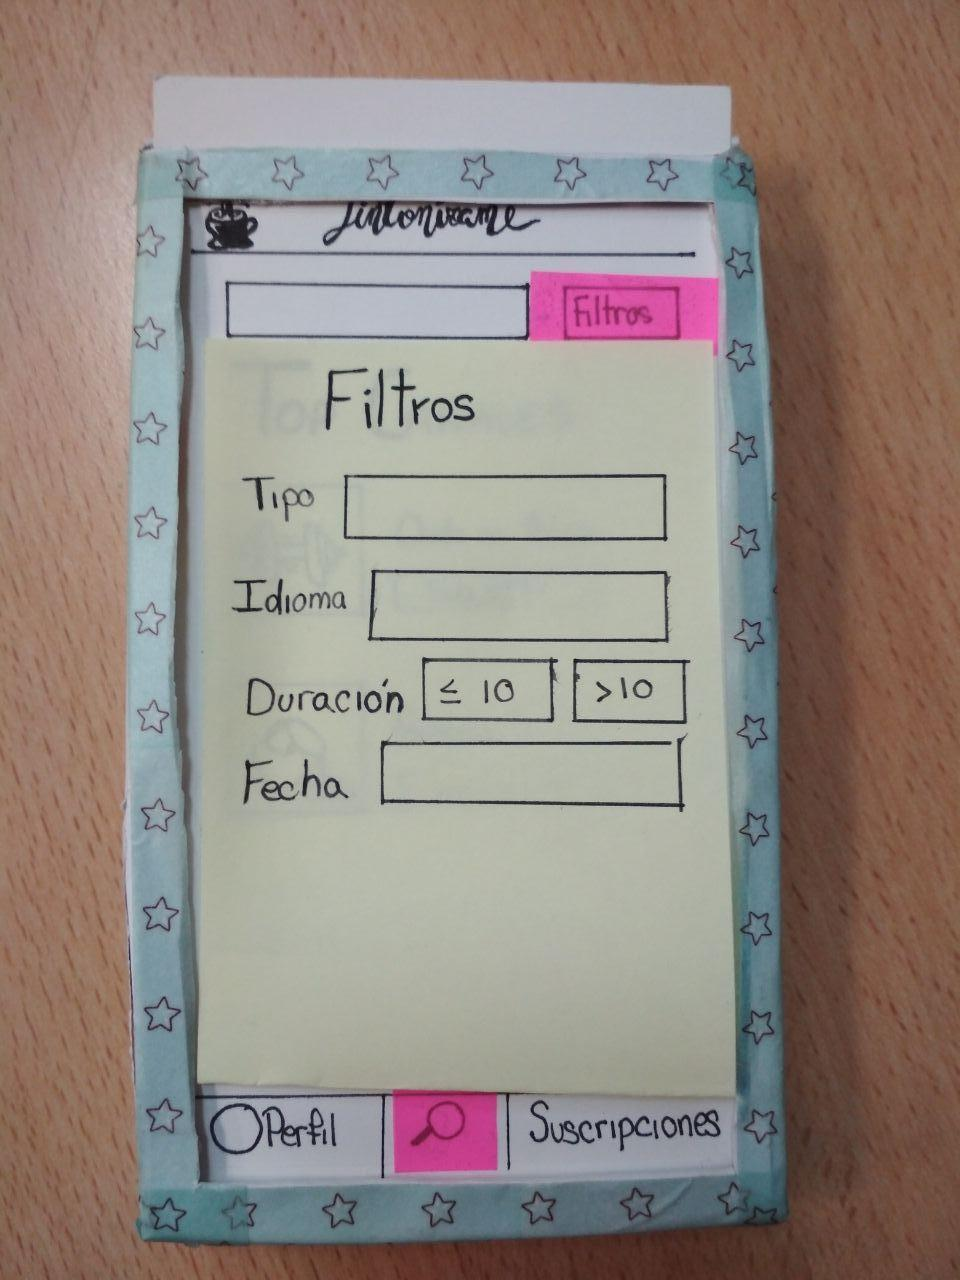
\includegraphics[width=0.4\columnwidth]{T3-10.jpg}
\caption{Acceder a filtros}
\label{fig:t3-5}
También podemos buscar un podcast o un canal siguiendo unos filtros para ello bastaría con pulsar el botón de filtros que se encuentra al lateral del área de texto del buscador.
\end{figure}
\begin{figure}[H]
\centering
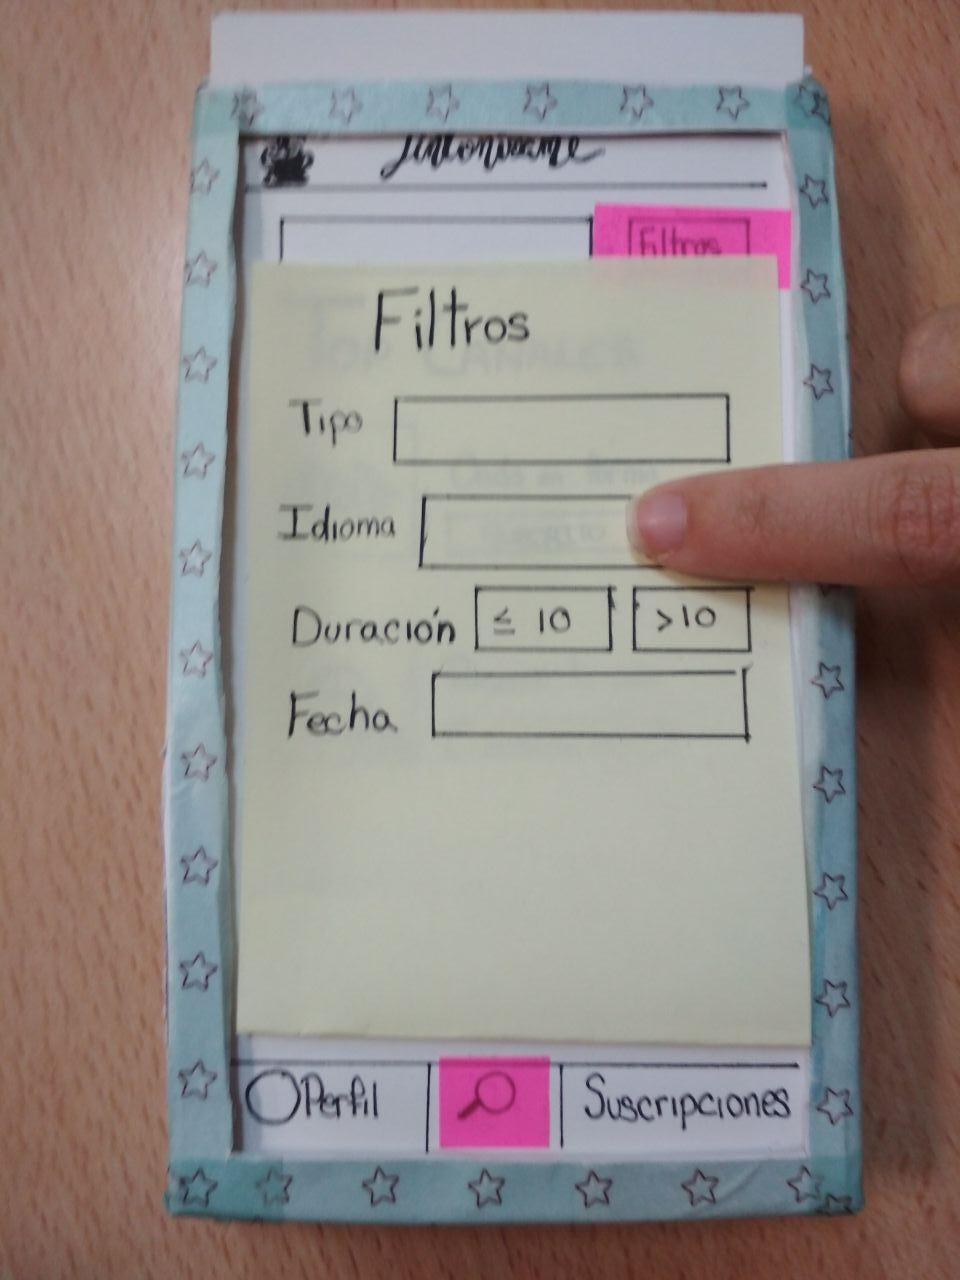
\includegraphics[width=0.4\columnwidth]{T3-9.jpg}
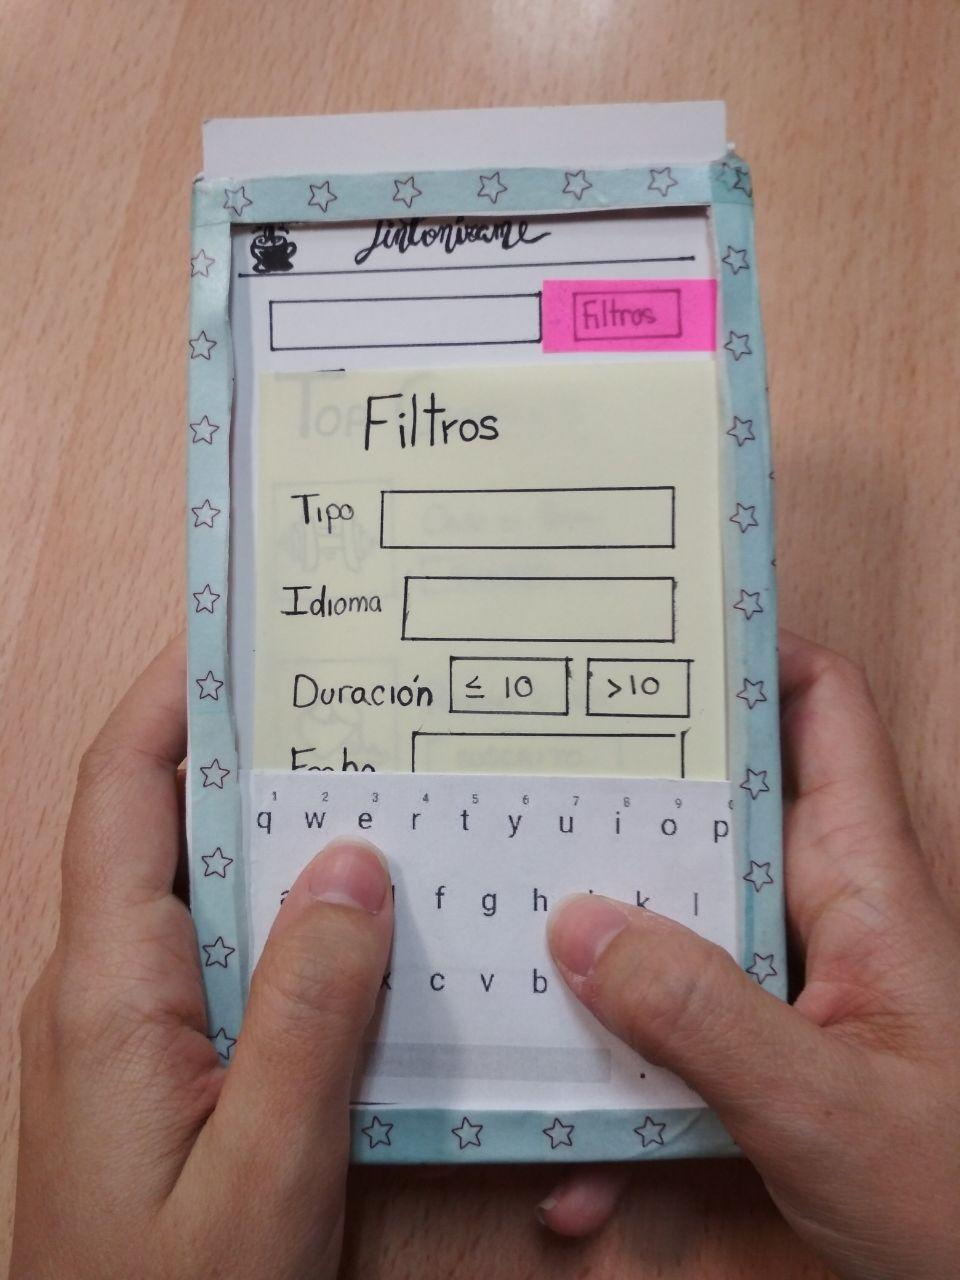
\includegraphics[width=0.4\columnwidth]{T3-8.jpg}
\caption{Introducir el filtro de idioma}
A través del teclado introducimos el idioma en el que queremos el podcast, en este caso seleccionaremos el español.
\label{fig:t3-7}
\end{figure}
\begin{figure}[H]
\centering
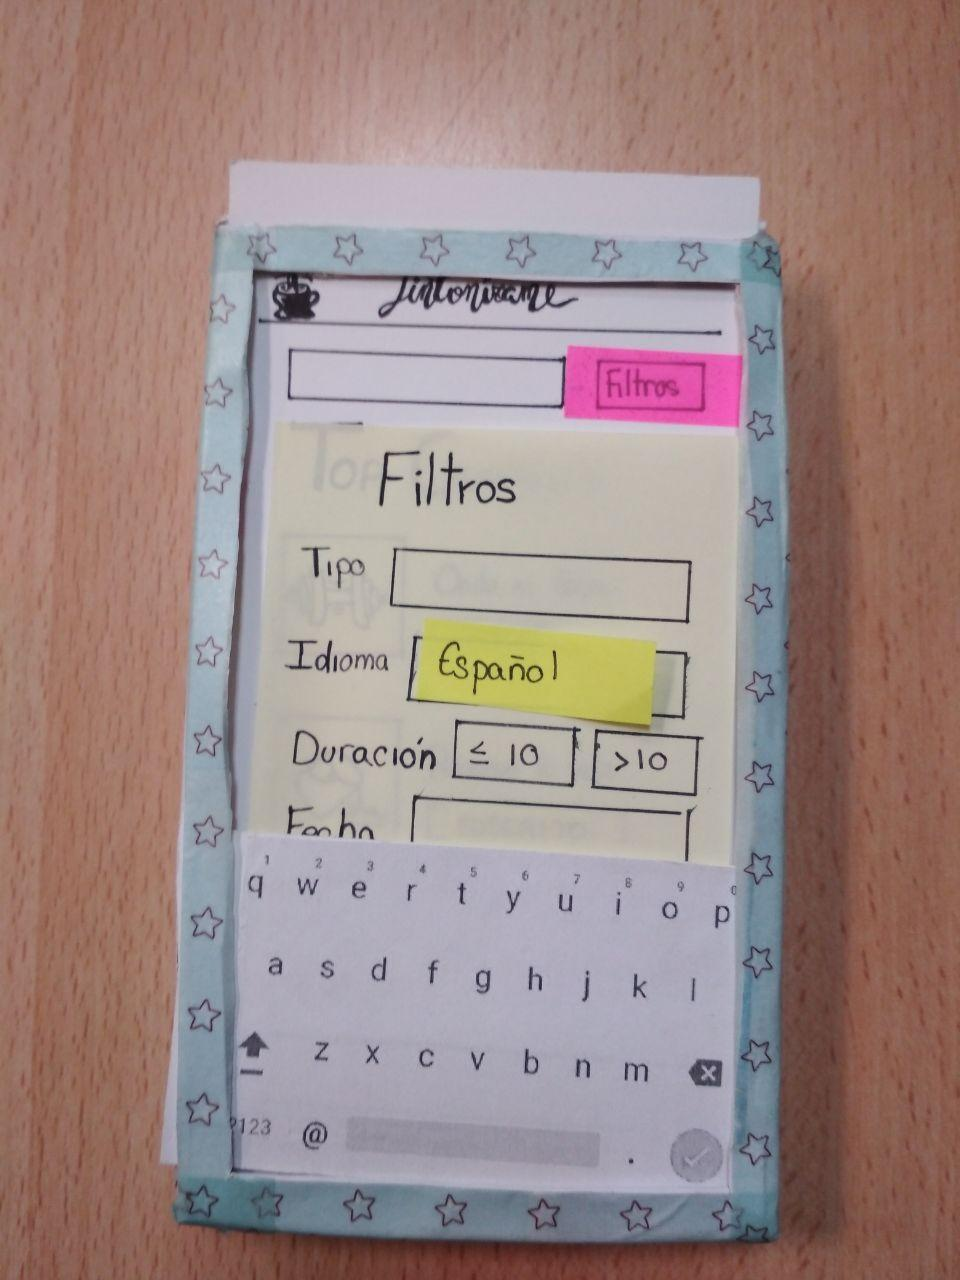
\includegraphics[width=0.4\columnwidth]{T3-7.jpg}
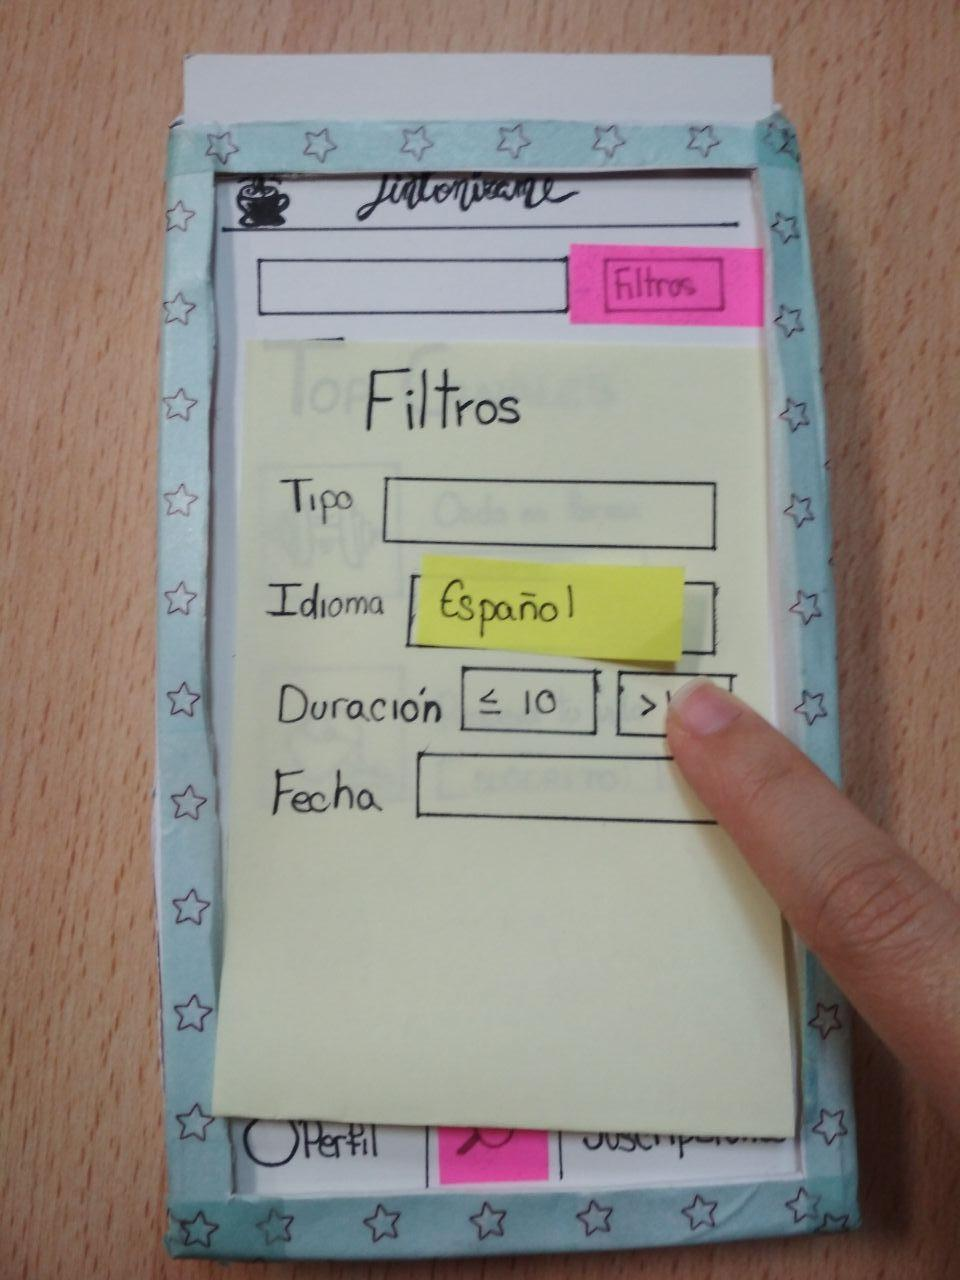
\includegraphics[width=0.4\columnwidth]{T3-6.jpg}
\caption{Introducir el filtro de duración}
\label{fig:t3-9}
\end{figure}
Dentro de los filtros se te permite elegir la duración del podcast en un intervalo menor o mayor a 10 minutos. En este caso hemos seleccionado un podcast con una duración mayor a 10 minutos.
\begin{figure}[H]
\centering
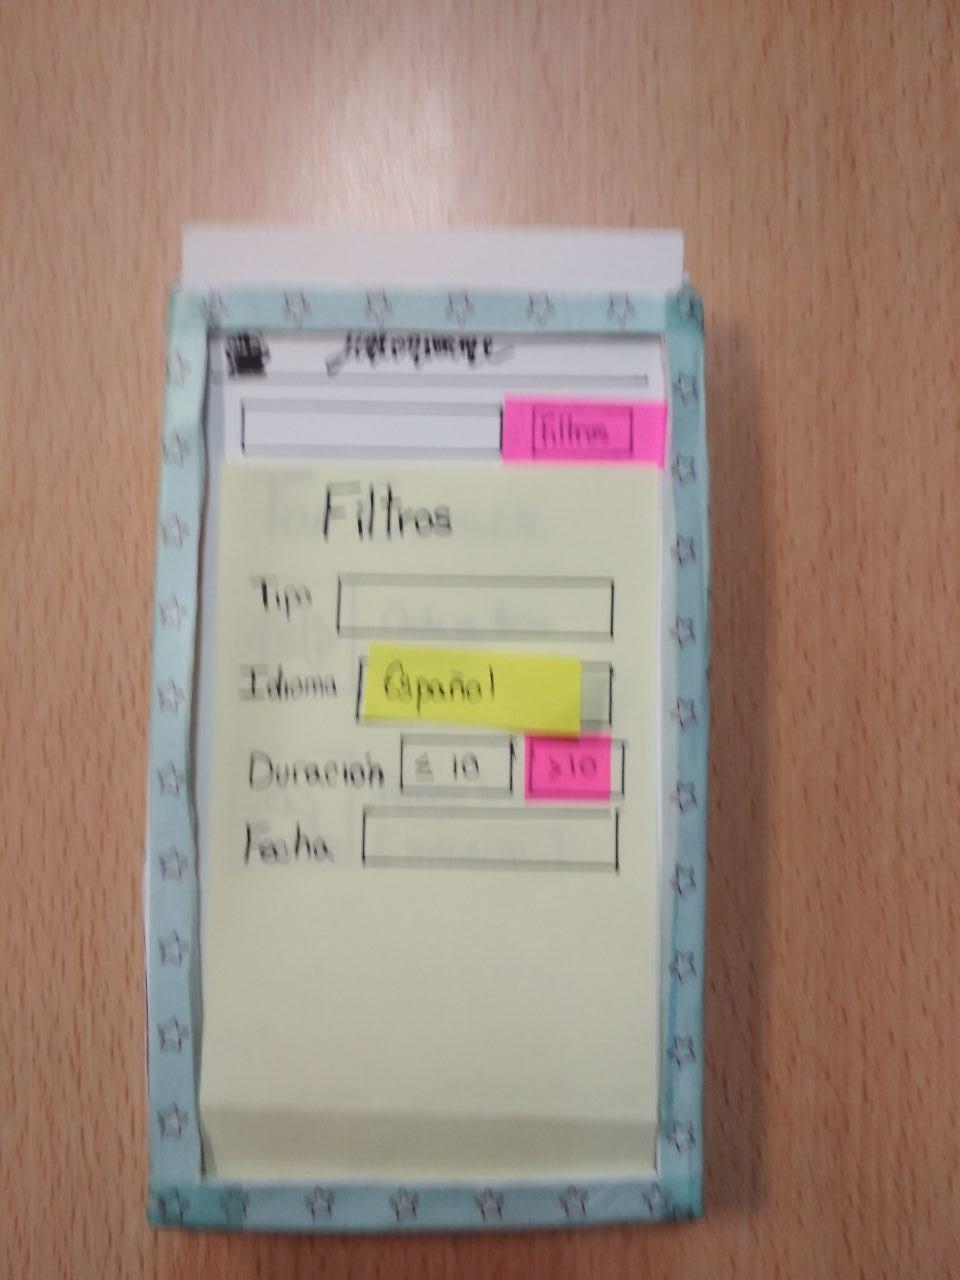
\includegraphics[width=0.4\columnwidth]{T3-5.jpg}
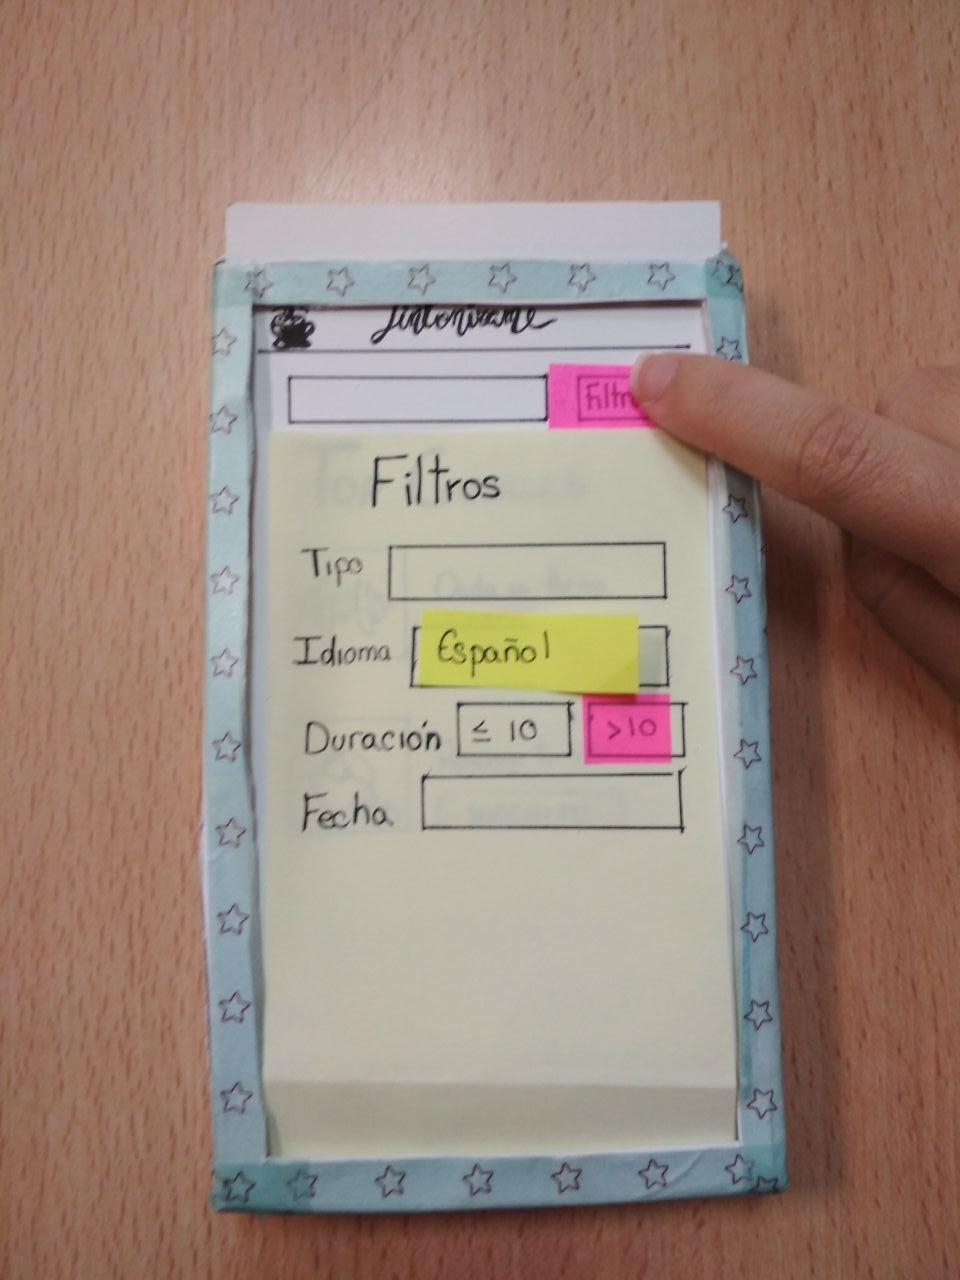
\includegraphics[width=0.4\columnwidth]{T3-4.jpg}
\caption{Cerrar filtros}
Cerramos los filtros volviendo a pulsar en el botón para deseleccionarlo.
\label{fig:t3-11}
\end{figure}
\begin{figure}[H]
\centering
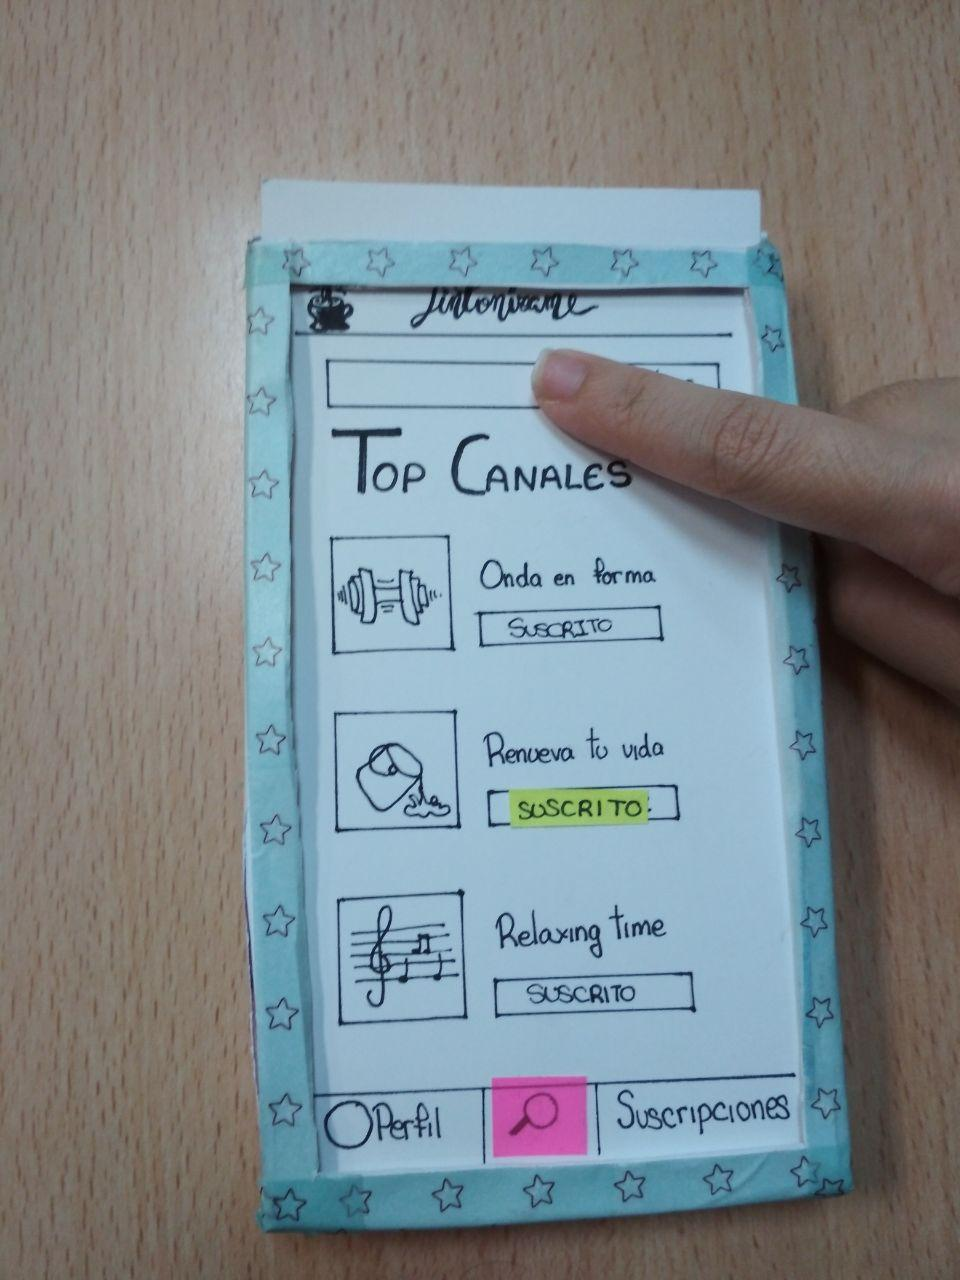
\includegraphics[width=0.4\columnwidth]{T3-15.jpg}
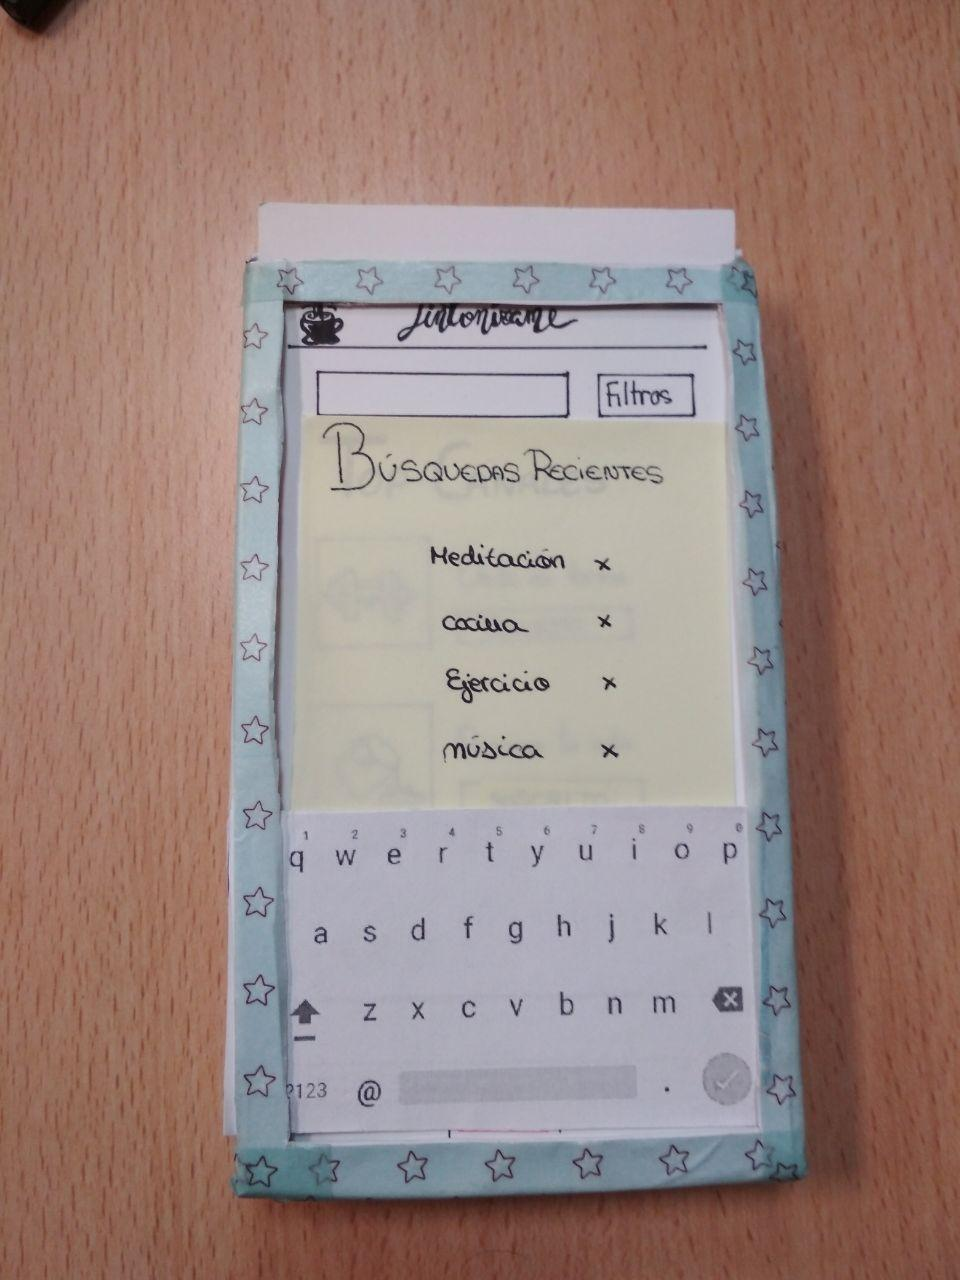
\includegraphics[width=0.4\columnwidth]{T3-14.jpg}
\caption{Barra de búsqueda}
\label{fig:t3-13}
\end{figure}
Si pulsamos en el área de texto del buscador nos saldrá automáticamente una lista de las búsquedas recientes y el teclado para poder escribir.
\begin{figure}[H]
\centering
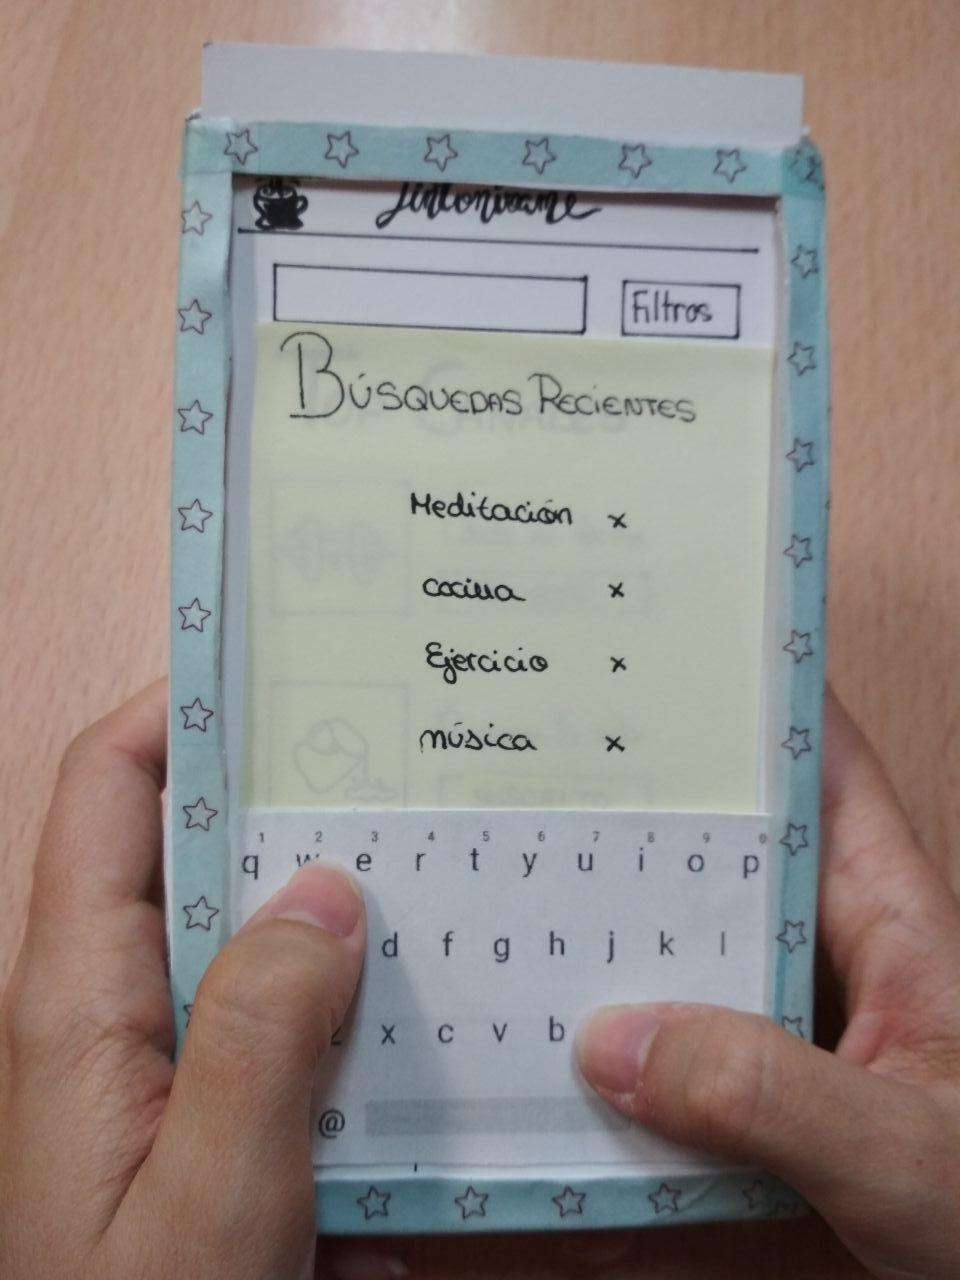
\includegraphics[width=0.4\columnwidth]{T3-13.jpg}
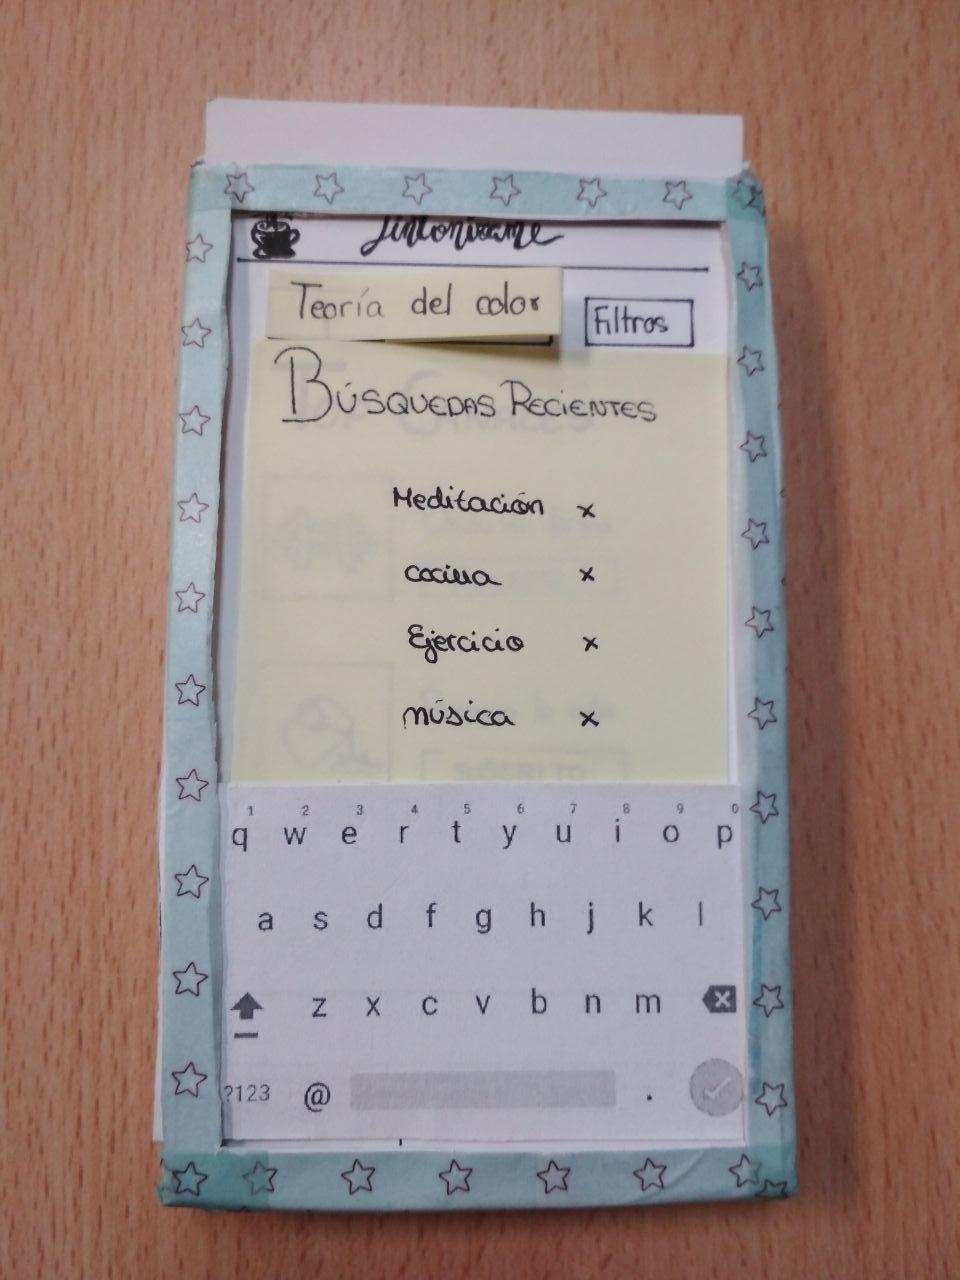
\includegraphics[width=0.4\columnwidth]{T3-12.jpg}
\caption{Introducción del nombre del podcast}
\label{fig:t3-15}
Podríamos haber elegido alguna de las temáticas que hemos buscado recientemente, pero en este caso la intención es buscar un podcast concreto sobre la teoría del color con los filtros seleccionados anteriormente.
\end{figure}
\begin{figure}[H]
\centering
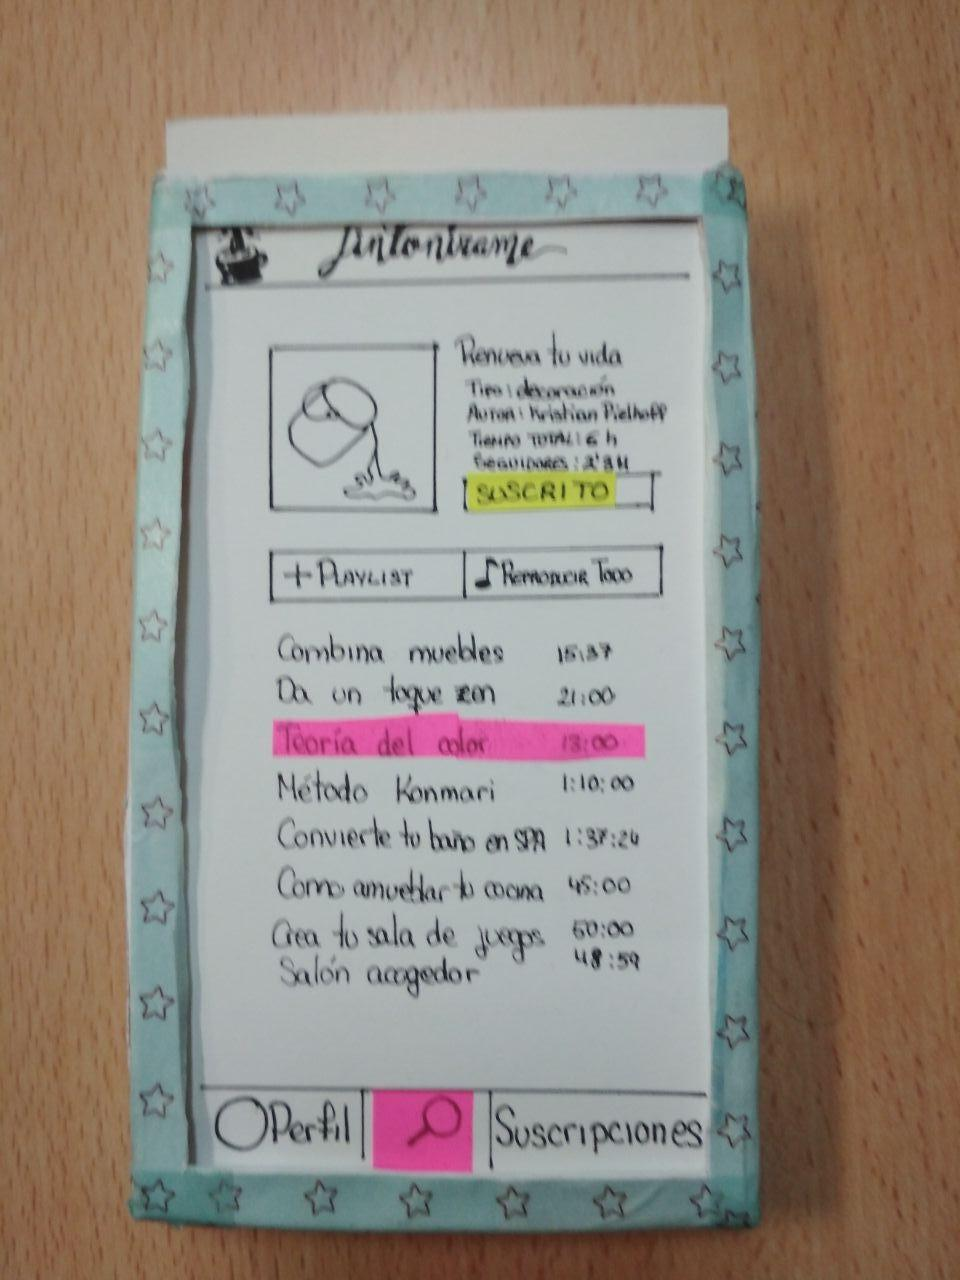
\includegraphics[width=0.4\columnwidth]{T3-3.jpg}
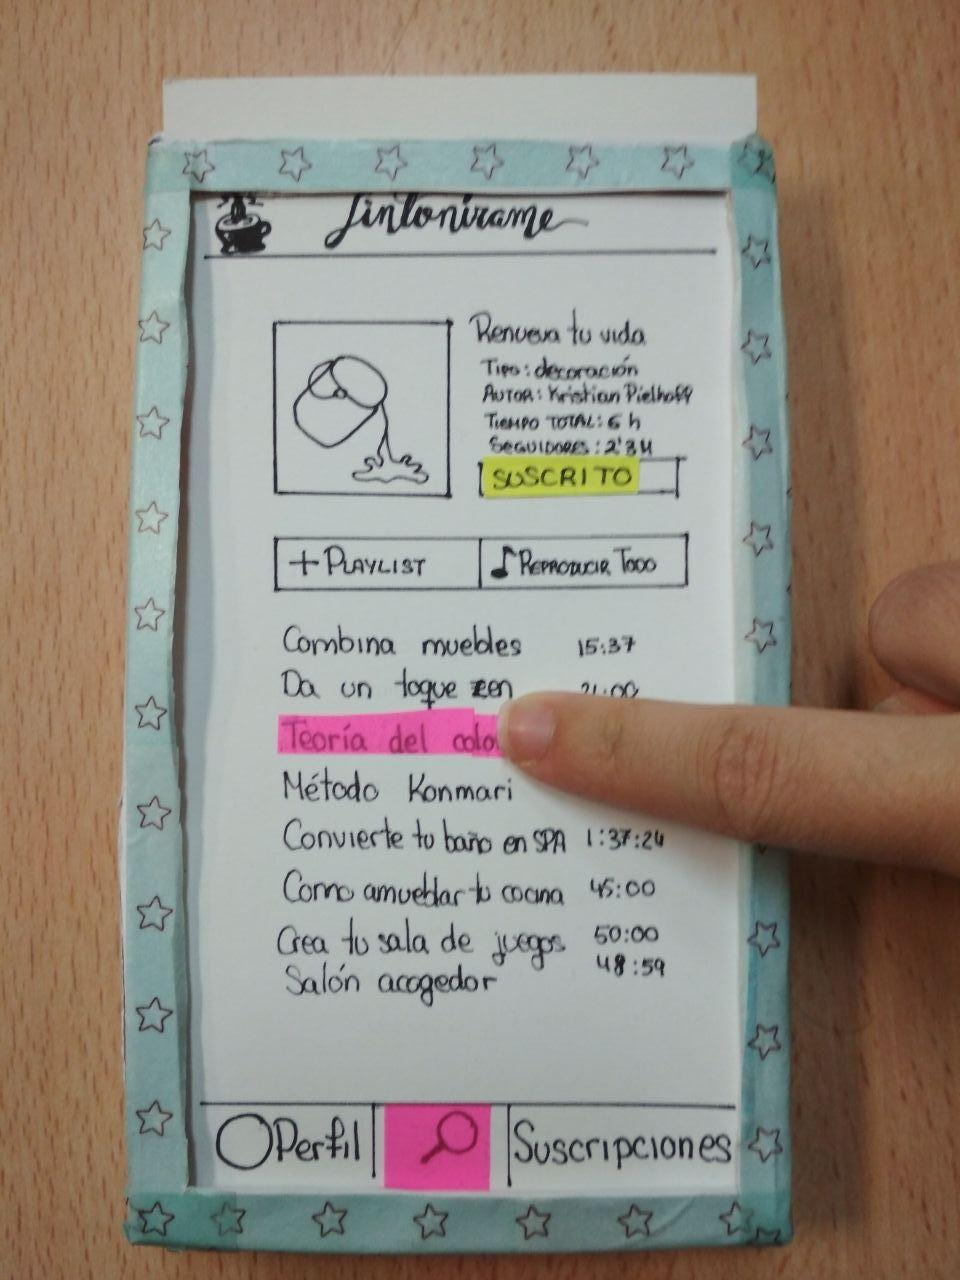
\includegraphics[width=0.4\columnwidth]{T3-2.jpg}
\caption{Selección del podcast}
\label{fig:t3-17}
Una vez introducida nuestra búsqueda la aplicación buscará un podcast que se adapte a nuestras expectativas y nos lo mostrará, pulsando sobre él será suficiente para empezar a reproducirlo.:
\end{figure}
\begin{figure}[H]
\centering
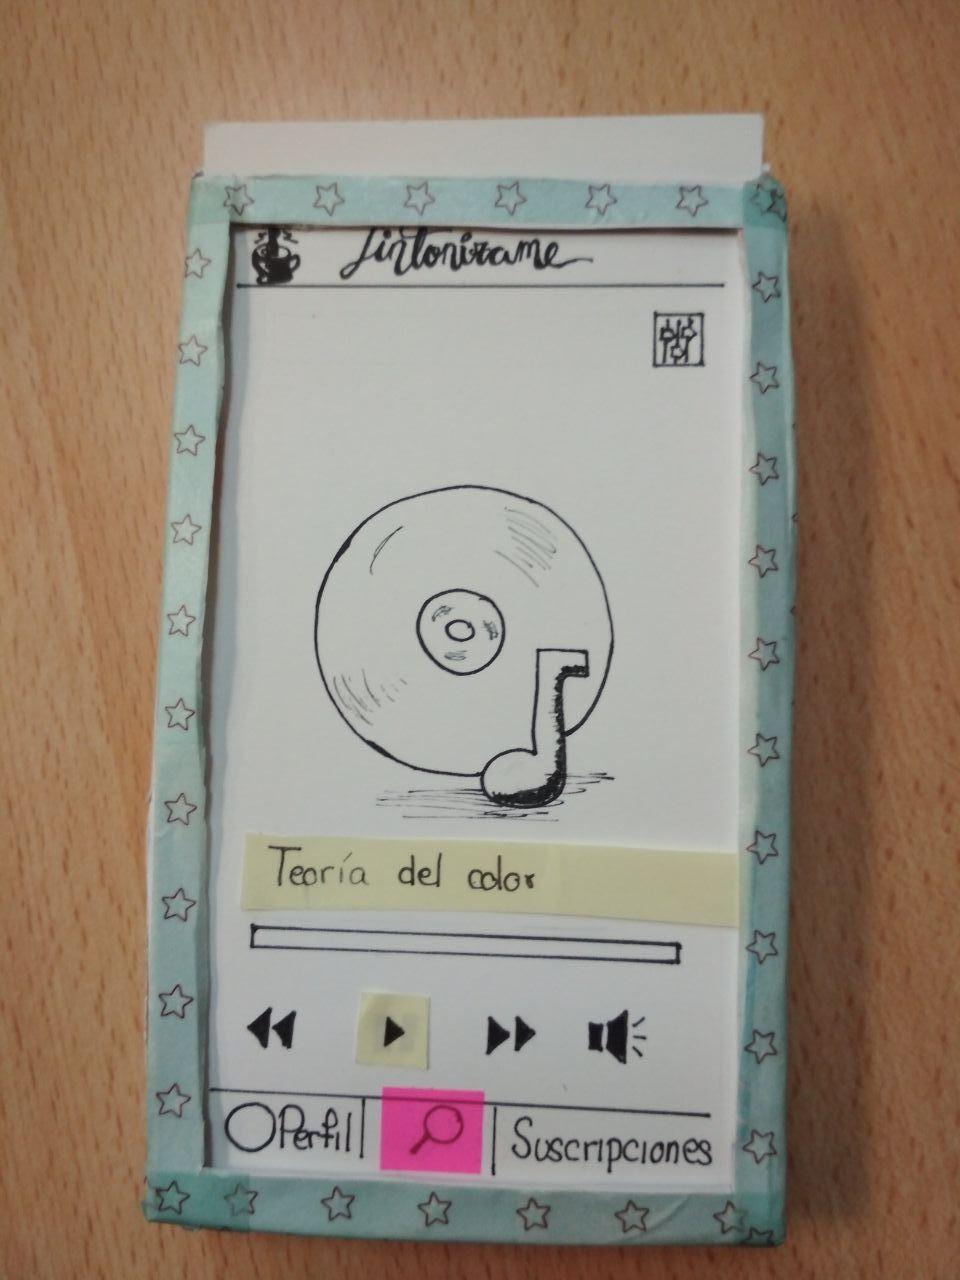
\includegraphics[width=0.4\columnwidth]{T3-1.jpg}
\caption{Reproducción del podcast}
\label{fig:t3-19}
El podcast inicialmente se encuentra en pause, para empezar a reproducirlo bastaría con pulsar el botón de play.
\end{figure}
\end{center}


\section{Bibliografía}

\begin{itemize}
\item Alejandra Martínez Monés, Apuntes asginatura IPC Universidad e Valladolid 2018
\item Jerónimo Pérez Paz, http://www.jeronimoperez.com/blog/diseno-web/ejemplo-de-test-de-usabilidad/ (visitado 16 de mayo de 2018)
\end{itemize}


\appendix

\section{Apéndices}

\subsection{Bocetos}
\label{bocetos}

\subsubsection{Bocetos móvil}
\begin{center}
\begin{figure}[H]
\centering
\caption{Bocetos móvil}
\label{fig:bm}
\end{figure}
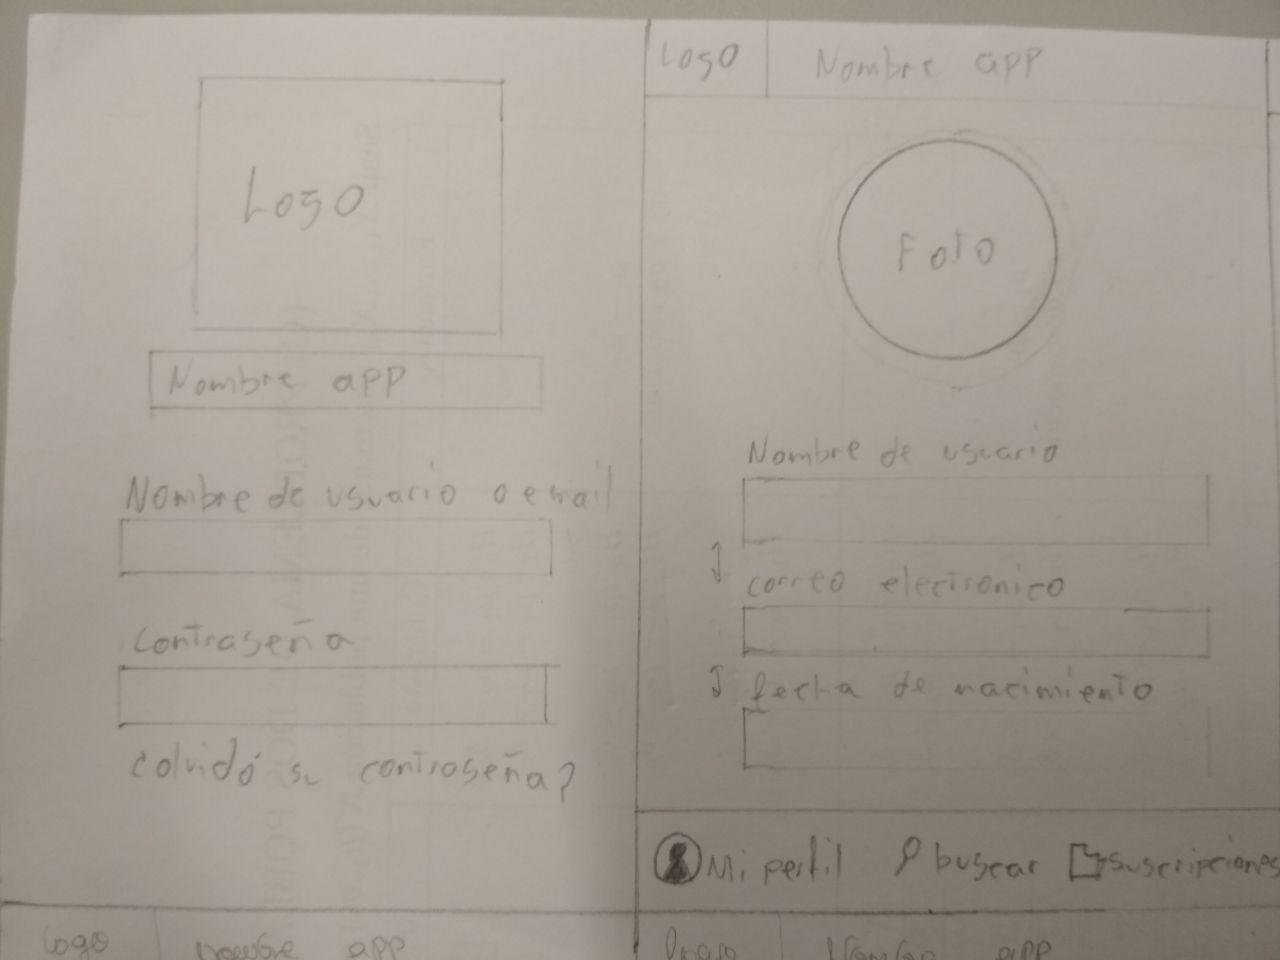
\includegraphics[width=0.7\columnwidth]{Boceto-1.jpg} \\
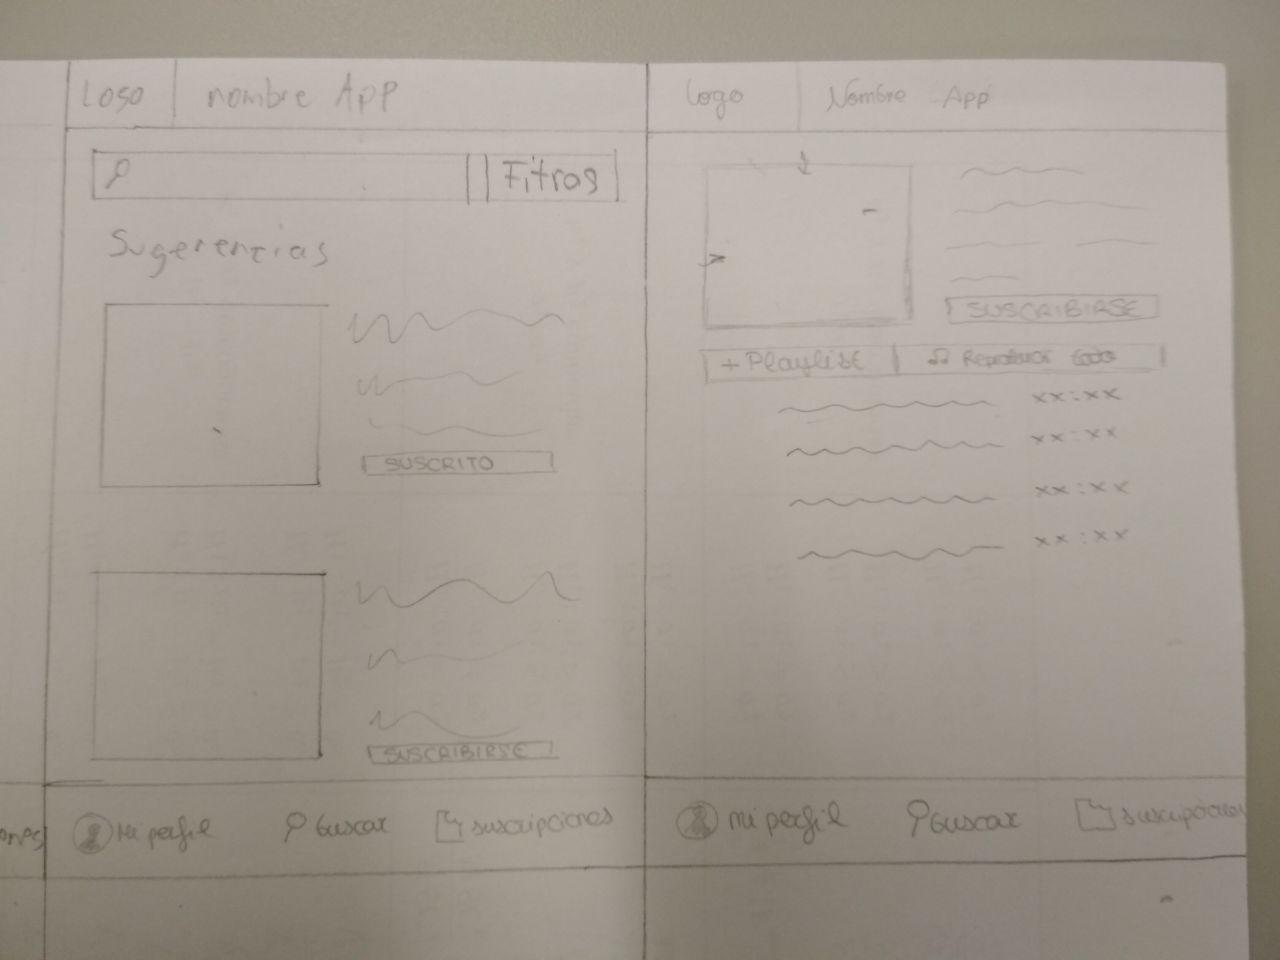
\includegraphics[width=0.7\columnwidth]{Boceto-2.jpg} \\
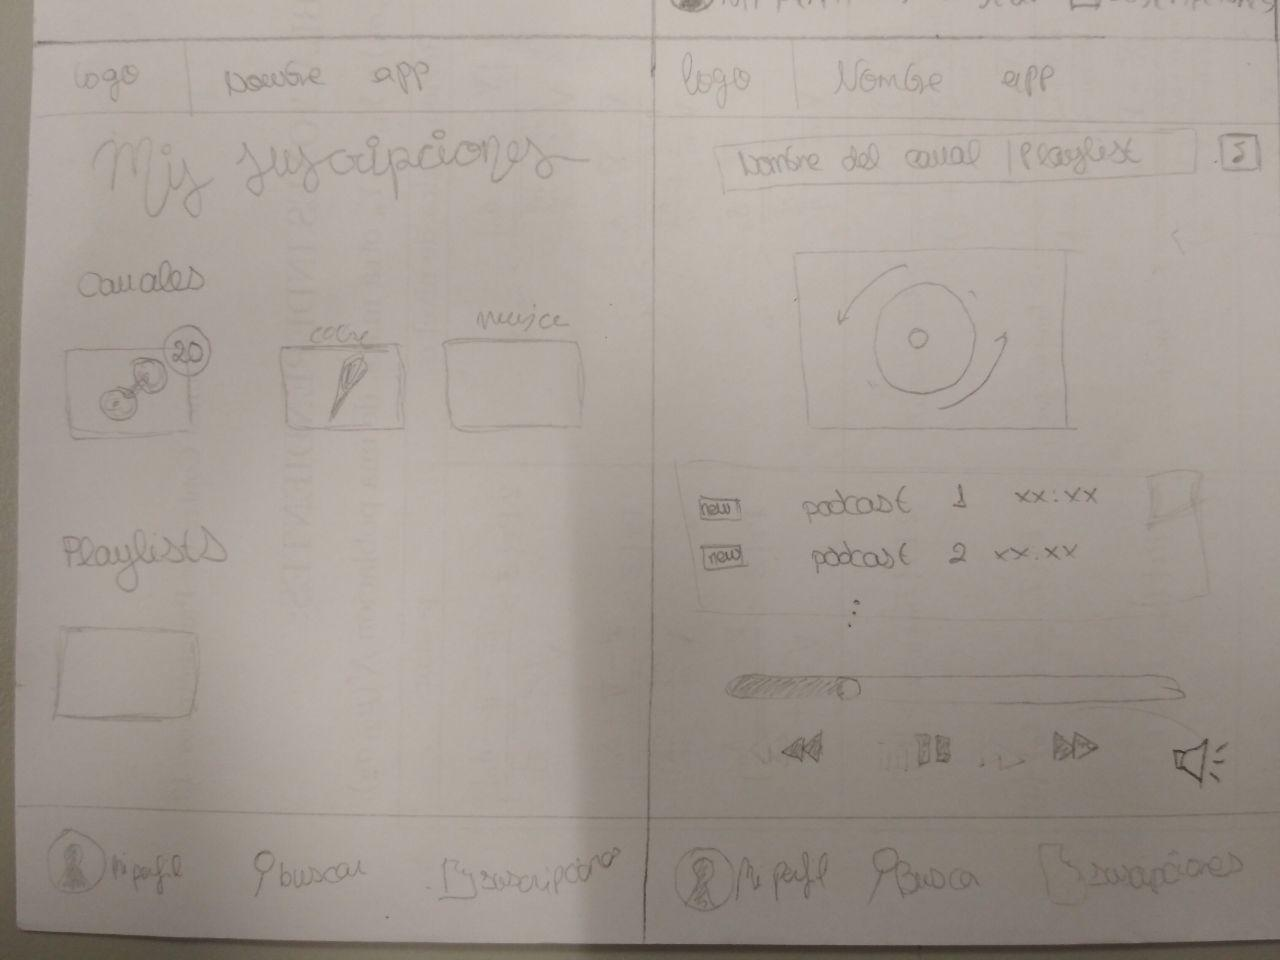
\includegraphics[width=0.7\columnwidth]{Boceto-3.jpg}
\end{center}
\subsubsection{Bocetos tablet y ordenador}
\begin{center}
\begin{figure}[H]
\centering
\caption{Bocetos tablet y ordenador}
\label{fig:bto}
\end{figure}
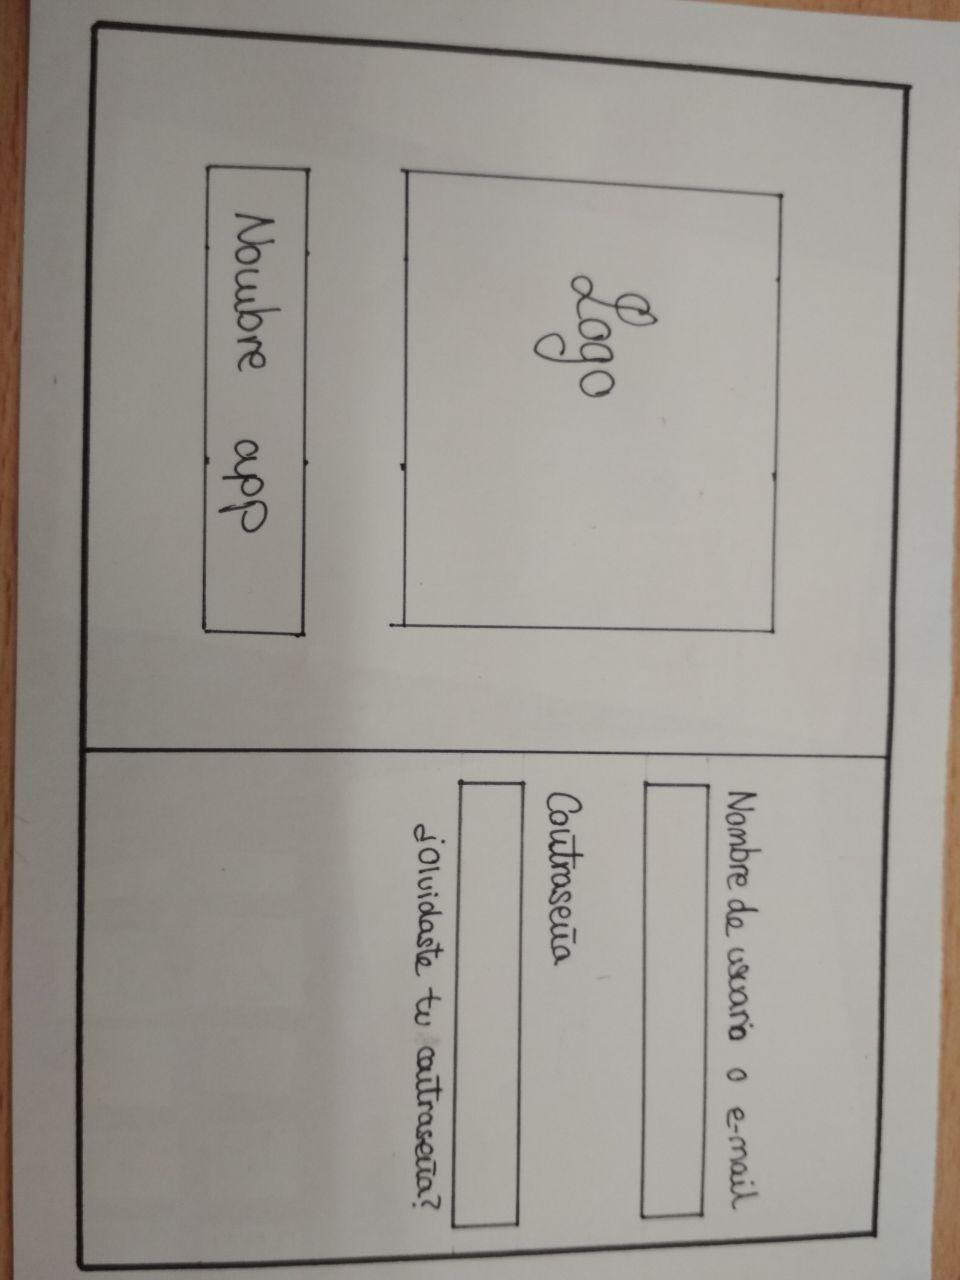
\includegraphics[width=0.7\columnwidth,angle=90]{Boceto4.jpg} \\
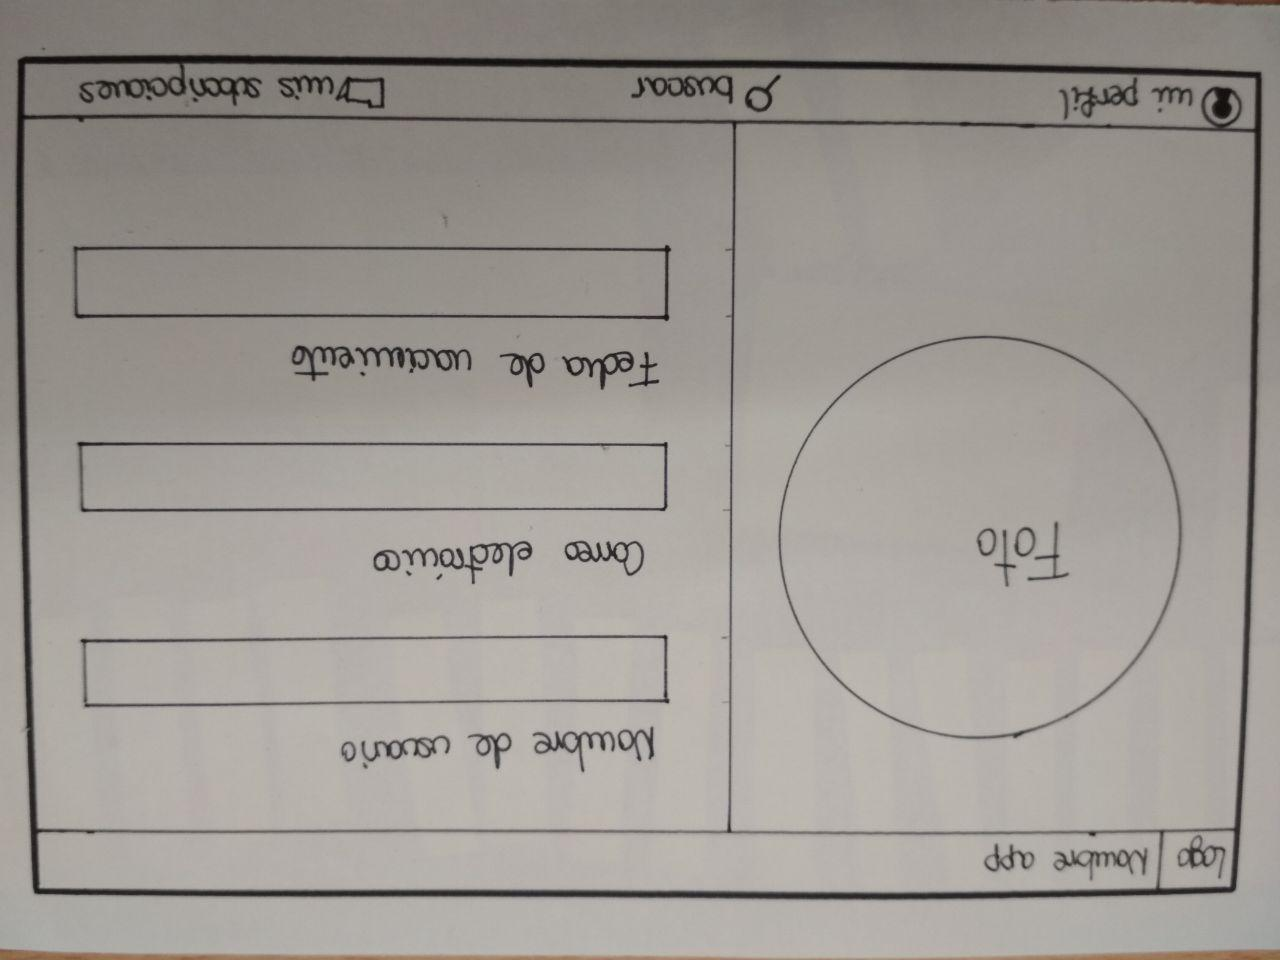
\includegraphics[width=0.7\columnwidth,angle=180]{Boceto5.jpg} \\
\includegraphics[width=0.7\columnwidth,angle=180]{Boceto6.jpg} \\
\includegraphics[width=0.7\columnwidth,angle=90]{Boceto7.jpg}
\end{center}

\end{document}
